% =============================================================================
% 04-registers-instructions.tex — Week 4: Register & Stack Organization,
% Instruction Set & Formats, Instruction Cycle, Types of Operands
%
% Course: Computer Organization and Architecture (PCC CS-401)
% Anchor reading: Mano Ch. 5 (Sec. 5-2, common bus system, p.127-129) and
%                 Mano Ch. 8 (CPU structure 8-1, register organization 8-2,
%                 stack organization 8-3, instruction formats 8-4) --
%                 page-cited where an index exists (see
%                 master_supporting_docs/CS401/supporting_books/Mano1993/index.md);
%                 Hamacher Ch. 7 (instruction cycle, operand types) --
%                 general/standard treatment, chapter-level, no page number
%                 (Hamacher index not yet built).
%
% Compile with: /compile-latex CS401/04-registers-instructions
% =============================================================================

\documentclass[aspectratio=169]{beamer}
% =============================================================================
% Preambles/header.tex — shared LaTeX/Beamer preamble for this project
%
% Use from a Beamer lecture by prepending:
%     % =============================================================================
% Preambles/header.tex — shared LaTeX/Beamer preamble for this project
%
% Use from a Beamer lecture by prepending:
%     % =============================================================================
% Preambles/header.tex — shared LaTeX/Beamer preamble for this project
%
% Use from a Beamer lecture by prepending:
%     \input{header}
% and compiling with TEXINPUTS=../Preambles:$TEXINPUTS (the /compile-latex
% skill does this automatically).
%
% PALETTE CONTRACT. Color names defined here MUST match the names in
% Quarto/theme-template.scss so Beamer and Quarto renderings use the same
% palette. The scripts/check-palette-sync.sh script enforces this.
%
% To customize: edit the HEX values below AND the matching $variable in
% Quarto/theme-template.scss, then run scripts/check-palette-sync.sh.
%
% TITLE PAGE. A formal, serif (Libertine) title-page template is defined in
% the Beamer-only block below (\setbeamertemplate{title page}) -- title,
% subtitle, a thin gold rule, then \author/\institute/\date. Frametitle and
% body text remain on Beamer's sans-serif default. No SCSS counterpart is
% needed for this (font/layout only, no new colors).
% =============================================================================

% -----------------------------------------------------------------------------
% Engine detection + encoding
%
% Our /compile-latex skill uses XeLaTeX, where inputenc is unnecessary and
% can produce encoding warnings. Only load inputenc under pdfTeX.
% -----------------------------------------------------------------------------
\usepackage{iftex}
\ifPDFTeX
  \usepackage[utf8]{inputenc}
\fi

\usepackage{amsmath, amssymb, amsthm}
\usepackage{booktabs}
\usepackage{graphicx}

% -----------------------------------------------------------------------------
% Serif face for the title page (formal/academic look). Linux Libertine is
% XeLaTeX- and pdfTeX-safe and redefines \rmdefault, so \rmfamily picks it up
% everywhere \rmfamily is used explicitly. Body text and frametitles stay on
% Beamer's own sans-serif default (unaffected) -- only the title-page
% \setbeamerfont{...} overrides below opt in to \rmfamily.
% -----------------------------------------------------------------------------
\usepackage{libertine}

% -----------------------------------------------------------------------------
% PALETTE — mirrors Quarto/theme-template.scss variable names.
% Load xcolor and define colors BEFORE anything that references them
% (notably hyperref, hypersetup, and the Beamer color assignments).
% -----------------------------------------------------------------------------
\usepackage{xcolor}

\definecolor{primary-blue}{HTML}{012169}      % headings, accents
\definecolor{primary-gold}{HTML}{B9975B}      % emphasis, borders
\definecolor{highlight-yellow}{HTML}{F2A900}  % markers, alerts
\definecolor{light-bg}{HTML}{E8EDF5}          % title / section backgrounds
\definecolor{jet}{HTML}{1A1A1A}               % body text

% Semantic colors (used in diagrams and annotations)
\definecolor{positive}{HTML}{15803D}          % good / observed / identified
\definecolor{negative}{HTML}{B91C1C}          % bad / problematic / bias
\definecolor{neutral}{HTML}{525252}           % reference / context

% Highlight accents (match .hi-* classes in the SCSS)
\definecolor{hi-slate}{HTML}{314F4F}
\definecolor{hi-green}{HTML}{2E8B57}
\definecolor{hi-red}{HTML}{C41E3A}

% Semantic aliases so skill templates and snippets can write
% \textcolor{accent}{...} without hard-coding "primary-blue".
\colorlet{accent}{primary-blue}
\colorlet{accent2}{primary-gold}

% -----------------------------------------------------------------------------
% Hyperref — loaded AFTER xcolor + palette so link colors resolve.
% -----------------------------------------------------------------------------
\usepackage{hyperref}
\hypersetup{colorlinks=true, linkcolor=primary-blue, urlcolor=primary-blue,
            citecolor=primary-blue, pdfborder={0 0 0}}

% -----------------------------------------------------------------------------
% Course code — set once per deck (after \input{header}, before \begin{document})
% via \coursecode{CS401}. Shown in the footer on every slide so a deck's course
% is identifiable without opening the title page. Empty by default.
% -----------------------------------------------------------------------------
\makeatletter
\newcommand{\coursecode}[1]{\gdef\@coursecodetext{#1}}
\gdef\@coursecodetext{}
\makeatother

% -----------------------------------------------------------------------------
% Beamer theme assignments (only apply under Beamer).
%
% We detect Beamer via \@ifclassloaded{beamer}, which is the documented,
% non-internal way. This must be wrapped in \makeatletter/\makeatother
% because \@ifclassloaded contains an @-catcode character.
% -----------------------------------------------------------------------------
\makeatletter
\@ifclassloaded{beamer}{%
  \usefonttheme{professionalfonts}
  \setbeamercolor{structure}{fg=primary-blue}
  \setbeamercolor{frametitle}{fg=primary-blue}
  \setbeamercolor{title}{fg=primary-blue}
  \setbeamercolor{subtitle}{fg=primary-gold}
  \setbeamercolor{author}{fg=primary-blue}
  \setbeamercolor{institute}{fg=neutral}
  \setbeamercolor{date}{fg=primary-gold}
  \setbeamercolor{itemize item}{fg=primary-blue}
  \setbeamercolor{itemize subitem}{fg=primary-gold}
  \setbeamercolor{alerted text}{fg=primary-gold}
  \setbeamercolor{block title}{fg=white, bg=primary-blue}
  \setbeamercolor{block body}{bg=light-bg}
  % Semantic block variants: block=definition/concept (blue), exampleblock=
  % worked example (green/positive), alertblock=key takeaway or caution (gold).
  % Keep to <=2 colored boxes per slide across ALL three variants (INV-7).
  \setbeamercolor{block title example}{fg=white, bg=positive}
  \setbeamercolor{block body example}{bg=light-bg}
  \setbeamercolor{block title alerted}{fg=white, bg=primary-gold}
  \setbeamercolor{block body alerted}{bg=light-bg}

  % ---------------------------------------------------------------------------
  % Formal title page: serif (Libertine, via \rmfamily) for title-page
  % elements only. Body text, itemize, and frametitle are intentionally left
  % on Beamer's sans-serif default -- \usebeamerfont{title} is also what
  % \transitionslide (below) uses for its big centered text, so section
  % transitions pick up the same serif treatment for free.
  % ---------------------------------------------------------------------------
  \setbeamerfont{title}{family=\rmfamily, series=\bfseries, size=\Large}
  \setbeamerfont{subtitle}{family=\rmfamily, shape=\itshape, size=\normalsize}
  \setbeamerfont{author}{family=\rmfamily, size=\normalsize}
  \setbeamerfont{institute}{family=\rmfamily, size=\scriptsize}
  \setbeamerfont{date}{family=\rmfamily, size=\scriptsize}

  \setbeamertemplate{title page}{
    \vfill
    \begin{center}
      {\usebeamerfont{title}\usebeamercolor[fg]{title}\inserttitle\par}
      \vspace{0.15cm}
      {\usebeamerfont{subtitle}\usebeamercolor[fg]{subtitle}\insertsubtitle\par}
      \vspace{0.45cm}
      {\color{primary-gold}\rule{0.42\textwidth}{0.6pt}\par}
      \vspace{0.45cm}
      {\usebeamerfont{author}\usebeamercolor[fg]{author}\insertauthor\par}
      \vspace{0.35cm}
      {\usebeamerfont{institute}\usebeamercolor[fg]{institute}\insertinstitute\par}
      \vspace{0.35cm}
      {\usebeamerfont{date}\usebeamercolor[fg]{date}\insertdate\par}
    \end{center}
    \vfill
  }

  % Minimal footer: course code (left) + page X / N (right), no navigation clutter
  \setbeamertemplate{navigation symbols}{}
  \setbeamertemplate{footline}{%
    \color{neutral}\footnotesize\hspace{0.7em}\@coursecodetext\hfill
    \insertframenumber/\inserttotalframenumber\hspace{0.7em}\vspace{0.3em}}
}{}
\makeatother

% -----------------------------------------------------------------------------
% TikZ setup — libraries the snippet gallery uses
% -----------------------------------------------------------------------------
\usepackage{tikz}
\usetikzlibrary{arrows.meta, positioning, calc, decorations.pathreplacing,
                fit, shapes.geometric, backgrounds}

% Shared TikZ styles — snippets and hand-written diagrams can pick these up
% via `\begin{tikzpicture}[every node/.style={...}]` or by naming specific
% styles (e.g., `\node[dag-node] (X) at (0,0) {X};`).
\tikzset{
  % Node styles for causal DAGs and similar
  dag-node/.style = {
    draw=primary-blue, fill=light-bg, rounded corners=2pt,
    minimum width=1.2cm, minimum height=0.9cm, align=center, font=\small
  },
  decision-node/.style = {
    draw=primary-gold, fill=white, diamond, aspect=1.8,
    minimum width=1.8cm, minimum height=1.2cm, align=center, font=\small,
    inner sep=1pt
  },
  % Edge styles — observed vs counterfactual
  observed-edge/.style = {-{Latex[length=2.5mm]}, thick, draw=jet},
  counterfactual-edge/.style = {-{Latex[length=2.5mm]}, thick, draw=neutral, dashed},
  confound-edge/.style = {-{Latex[length=2.5mm]}, thick, draw=negative, dashed},
  % Data-point styles for plots
  observed-dot/.style = {fill=primary-blue, draw=primary-blue, circle, inner sep=1.2pt},
  counterfactual-dot/.style = {fill=white, draw=neutral, circle, inner sep=1.2pt}
}

% -----------------------------------------------------------------------------
% Convenience macros
% -----------------------------------------------------------------------------
\newcommand{\muted}[1]{\textcolor{neutral}{#1}}
\newcommand{\key}[1]{\textcolor{primary-gold}{\textbf{#1}}}
\newcommand{\good}[1]{\textcolor{positive}{#1}}
\newcommand{\bad}[1]{\textcolor{negative}{#1}}

% Standout frame macro: full-bleed dark background for section transitions.
% Beamer-only (uses \begin{frame}/\setbeamercolor/\usebeamerfont) -- do not
% call from an article-class file (e.g. Notes/<CODE>/*-notes.tex). \muted,
% \key, \good, \bad, and \coursecode above are plain xcolor/gdef and are
% safe to use from either class; verified when Notes/article-class support
% was added.
% Expand: \transitionslide{Your transition title}
\newcommand{\transitionslide}[1]{%
  \begingroup
  \setbeamercolor{background canvas}{bg=primary-blue}
  \begin{frame}[plain]
    \centering
    \vfill
    {\usebeamerfont{title}\color{white}\Large #1\par}
    \vfill
  \end{frame}
  \endgroup
}

% and compiling with TEXINPUTS=../Preambles:$TEXINPUTS (the /compile-latex
% skill does this automatically).
%
% PALETTE CONTRACT. Color names defined here MUST match the names in
% Quarto/theme-template.scss so Beamer and Quarto renderings use the same
% palette. The scripts/check-palette-sync.sh script enforces this.
%
% To customize: edit the HEX values below AND the matching $variable in
% Quarto/theme-template.scss, then run scripts/check-palette-sync.sh.
%
% TITLE PAGE. A formal, serif (Libertine) title-page template is defined in
% the Beamer-only block below (\setbeamertemplate{title page}) -- title,
% subtitle, a thin gold rule, then \author/\institute/\date. Frametitle and
% body text remain on Beamer's sans-serif default. No SCSS counterpart is
% needed for this (font/layout only, no new colors).
% =============================================================================

% -----------------------------------------------------------------------------
% Engine detection + encoding
%
% Our /compile-latex skill uses XeLaTeX, where inputenc is unnecessary and
% can produce encoding warnings. Only load inputenc under pdfTeX.
% -----------------------------------------------------------------------------
\usepackage{iftex}
\ifPDFTeX
  \usepackage[utf8]{inputenc}
\fi

\usepackage{amsmath, amssymb, amsthm}
\usepackage{booktabs}
\usepackage{graphicx}

% -----------------------------------------------------------------------------
% Serif face for the title page (formal/academic look). Linux Libertine is
% XeLaTeX- and pdfTeX-safe and redefines \rmdefault, so \rmfamily picks it up
% everywhere \rmfamily is used explicitly. Body text and frametitles stay on
% Beamer's own sans-serif default (unaffected) -- only the title-page
% \setbeamerfont{...} overrides below opt in to \rmfamily.
% -----------------------------------------------------------------------------
\usepackage{libertine}

% -----------------------------------------------------------------------------
% PALETTE — mirrors Quarto/theme-template.scss variable names.
% Load xcolor and define colors BEFORE anything that references them
% (notably hyperref, hypersetup, and the Beamer color assignments).
% -----------------------------------------------------------------------------
\usepackage{xcolor}

\definecolor{primary-blue}{HTML}{012169}      % headings, accents
\definecolor{primary-gold}{HTML}{B9975B}      % emphasis, borders
\definecolor{highlight-yellow}{HTML}{F2A900}  % markers, alerts
\definecolor{light-bg}{HTML}{E8EDF5}          % title / section backgrounds
\definecolor{jet}{HTML}{1A1A1A}               % body text

% Semantic colors (used in diagrams and annotations)
\definecolor{positive}{HTML}{15803D}          % good / observed / identified
\definecolor{negative}{HTML}{B91C1C}          % bad / problematic / bias
\definecolor{neutral}{HTML}{525252}           % reference / context

% Highlight accents (match .hi-* classes in the SCSS)
\definecolor{hi-slate}{HTML}{314F4F}
\definecolor{hi-green}{HTML}{2E8B57}
\definecolor{hi-red}{HTML}{C41E3A}

% Semantic aliases so skill templates and snippets can write
% \textcolor{accent}{...} without hard-coding "primary-blue".
\colorlet{accent}{primary-blue}
\colorlet{accent2}{primary-gold}

% -----------------------------------------------------------------------------
% Hyperref — loaded AFTER xcolor + palette so link colors resolve.
% -----------------------------------------------------------------------------
\usepackage{hyperref}
\hypersetup{colorlinks=true, linkcolor=primary-blue, urlcolor=primary-blue,
            citecolor=primary-blue, pdfborder={0 0 0}}

% -----------------------------------------------------------------------------
% Course code — set once per deck (after % =============================================================================
% Preambles/header.tex — shared LaTeX/Beamer preamble for this project
%
% Use from a Beamer lecture by prepending:
%     \input{header}
% and compiling with TEXINPUTS=../Preambles:$TEXINPUTS (the /compile-latex
% skill does this automatically).
%
% PALETTE CONTRACT. Color names defined here MUST match the names in
% Quarto/theme-template.scss so Beamer and Quarto renderings use the same
% palette. The scripts/check-palette-sync.sh script enforces this.
%
% To customize: edit the HEX values below AND the matching $variable in
% Quarto/theme-template.scss, then run scripts/check-palette-sync.sh.
%
% TITLE PAGE. A formal, serif (Libertine) title-page template is defined in
% the Beamer-only block below (\setbeamertemplate{title page}) -- title,
% subtitle, a thin gold rule, then \author/\institute/\date. Frametitle and
% body text remain on Beamer's sans-serif default. No SCSS counterpart is
% needed for this (font/layout only, no new colors).
% =============================================================================

% -----------------------------------------------------------------------------
% Engine detection + encoding
%
% Our /compile-latex skill uses XeLaTeX, where inputenc is unnecessary and
% can produce encoding warnings. Only load inputenc under pdfTeX.
% -----------------------------------------------------------------------------
\usepackage{iftex}
\ifPDFTeX
  \usepackage[utf8]{inputenc}
\fi

\usepackage{amsmath, amssymb, amsthm}
\usepackage{booktabs}
\usepackage{graphicx}

% -----------------------------------------------------------------------------
% Serif face for the title page (formal/academic look). Linux Libertine is
% XeLaTeX- and pdfTeX-safe and redefines \rmdefault, so \rmfamily picks it up
% everywhere \rmfamily is used explicitly. Body text and frametitles stay on
% Beamer's own sans-serif default (unaffected) -- only the title-page
% \setbeamerfont{...} overrides below opt in to \rmfamily.
% -----------------------------------------------------------------------------
\usepackage{libertine}

% -----------------------------------------------------------------------------
% PALETTE — mirrors Quarto/theme-template.scss variable names.
% Load xcolor and define colors BEFORE anything that references them
% (notably hyperref, hypersetup, and the Beamer color assignments).
% -----------------------------------------------------------------------------
\usepackage{xcolor}

\definecolor{primary-blue}{HTML}{012169}      % headings, accents
\definecolor{primary-gold}{HTML}{B9975B}      % emphasis, borders
\definecolor{highlight-yellow}{HTML}{F2A900}  % markers, alerts
\definecolor{light-bg}{HTML}{E8EDF5}          % title / section backgrounds
\definecolor{jet}{HTML}{1A1A1A}               % body text

% Semantic colors (used in diagrams and annotations)
\definecolor{positive}{HTML}{15803D}          % good / observed / identified
\definecolor{negative}{HTML}{B91C1C}          % bad / problematic / bias
\definecolor{neutral}{HTML}{525252}           % reference / context

% Highlight accents (match .hi-* classes in the SCSS)
\definecolor{hi-slate}{HTML}{314F4F}
\definecolor{hi-green}{HTML}{2E8B57}
\definecolor{hi-red}{HTML}{C41E3A}

% Semantic aliases so skill templates and snippets can write
% \textcolor{accent}{...} without hard-coding "primary-blue".
\colorlet{accent}{primary-blue}
\colorlet{accent2}{primary-gold}

% -----------------------------------------------------------------------------
% Hyperref — loaded AFTER xcolor + palette so link colors resolve.
% -----------------------------------------------------------------------------
\usepackage{hyperref}
\hypersetup{colorlinks=true, linkcolor=primary-blue, urlcolor=primary-blue,
            citecolor=primary-blue, pdfborder={0 0 0}}

% -----------------------------------------------------------------------------
% Course code — set once per deck (after \input{header}, before \begin{document})
% via \coursecode{CS401}. Shown in the footer on every slide so a deck's course
% is identifiable without opening the title page. Empty by default.
% -----------------------------------------------------------------------------
\makeatletter
\newcommand{\coursecode}[1]{\gdef\@coursecodetext{#1}}
\gdef\@coursecodetext{}
\makeatother

% -----------------------------------------------------------------------------
% Beamer theme assignments (only apply under Beamer).
%
% We detect Beamer via \@ifclassloaded{beamer}, which is the documented,
% non-internal way. This must be wrapped in \makeatletter/\makeatother
% because \@ifclassloaded contains an @-catcode character.
% -----------------------------------------------------------------------------
\makeatletter
\@ifclassloaded{beamer}{%
  \usefonttheme{professionalfonts}
  \setbeamercolor{structure}{fg=primary-blue}
  \setbeamercolor{frametitle}{fg=primary-blue}
  \setbeamercolor{title}{fg=primary-blue}
  \setbeamercolor{subtitle}{fg=primary-gold}
  \setbeamercolor{author}{fg=primary-blue}
  \setbeamercolor{institute}{fg=neutral}
  \setbeamercolor{date}{fg=primary-gold}
  \setbeamercolor{itemize item}{fg=primary-blue}
  \setbeamercolor{itemize subitem}{fg=primary-gold}
  \setbeamercolor{alerted text}{fg=primary-gold}
  \setbeamercolor{block title}{fg=white, bg=primary-blue}
  \setbeamercolor{block body}{bg=light-bg}
  % Semantic block variants: block=definition/concept (blue), exampleblock=
  % worked example (green/positive), alertblock=key takeaway or caution (gold).
  % Keep to <=2 colored boxes per slide across ALL three variants (INV-7).
  \setbeamercolor{block title example}{fg=white, bg=positive}
  \setbeamercolor{block body example}{bg=light-bg}
  \setbeamercolor{block title alerted}{fg=white, bg=primary-gold}
  \setbeamercolor{block body alerted}{bg=light-bg}

  % ---------------------------------------------------------------------------
  % Formal title page: serif (Libertine, via \rmfamily) for title-page
  % elements only. Body text, itemize, and frametitle are intentionally left
  % on Beamer's sans-serif default -- \usebeamerfont{title} is also what
  % \transitionslide (below) uses for its big centered text, so section
  % transitions pick up the same serif treatment for free.
  % ---------------------------------------------------------------------------
  \setbeamerfont{title}{family=\rmfamily, series=\bfseries, size=\Large}
  \setbeamerfont{subtitle}{family=\rmfamily, shape=\itshape, size=\normalsize}
  \setbeamerfont{author}{family=\rmfamily, size=\normalsize}
  \setbeamerfont{institute}{family=\rmfamily, size=\scriptsize}
  \setbeamerfont{date}{family=\rmfamily, size=\scriptsize}

  \setbeamertemplate{title page}{
    \vfill
    \begin{center}
      {\usebeamerfont{title}\usebeamercolor[fg]{title}\inserttitle\par}
      \vspace{0.15cm}
      {\usebeamerfont{subtitle}\usebeamercolor[fg]{subtitle}\insertsubtitle\par}
      \vspace{0.45cm}
      {\color{primary-gold}\rule{0.42\textwidth}{0.6pt}\par}
      \vspace{0.45cm}
      {\usebeamerfont{author}\usebeamercolor[fg]{author}\insertauthor\par}
      \vspace{0.35cm}
      {\usebeamerfont{institute}\usebeamercolor[fg]{institute}\insertinstitute\par}
      \vspace{0.35cm}
      {\usebeamerfont{date}\usebeamercolor[fg]{date}\insertdate\par}
    \end{center}
    \vfill
  }

  % Minimal footer: course code (left) + page X / N (right), no navigation clutter
  \setbeamertemplate{navigation symbols}{}
  \setbeamertemplate{footline}{%
    \color{neutral}\footnotesize\hspace{0.7em}\@coursecodetext\hfill
    \insertframenumber/\inserttotalframenumber\hspace{0.7em}\vspace{0.3em}}
}{}
\makeatother

% -----------------------------------------------------------------------------
% TikZ setup — libraries the snippet gallery uses
% -----------------------------------------------------------------------------
\usepackage{tikz}
\usetikzlibrary{arrows.meta, positioning, calc, decorations.pathreplacing,
                fit, shapes.geometric, backgrounds}

% Shared TikZ styles — snippets and hand-written diagrams can pick these up
% via `\begin{tikzpicture}[every node/.style={...}]` or by naming specific
% styles (e.g., `\node[dag-node] (X) at (0,0) {X};`).
\tikzset{
  % Node styles for causal DAGs and similar
  dag-node/.style = {
    draw=primary-blue, fill=light-bg, rounded corners=2pt,
    minimum width=1.2cm, minimum height=0.9cm, align=center, font=\small
  },
  decision-node/.style = {
    draw=primary-gold, fill=white, diamond, aspect=1.8,
    minimum width=1.8cm, minimum height=1.2cm, align=center, font=\small,
    inner sep=1pt
  },
  % Edge styles — observed vs counterfactual
  observed-edge/.style = {-{Latex[length=2.5mm]}, thick, draw=jet},
  counterfactual-edge/.style = {-{Latex[length=2.5mm]}, thick, draw=neutral, dashed},
  confound-edge/.style = {-{Latex[length=2.5mm]}, thick, draw=negative, dashed},
  % Data-point styles for plots
  observed-dot/.style = {fill=primary-blue, draw=primary-blue, circle, inner sep=1.2pt},
  counterfactual-dot/.style = {fill=white, draw=neutral, circle, inner sep=1.2pt}
}

% -----------------------------------------------------------------------------
% Convenience macros
% -----------------------------------------------------------------------------
\newcommand{\muted}[1]{\textcolor{neutral}{#1}}
\newcommand{\key}[1]{\textcolor{primary-gold}{\textbf{#1}}}
\newcommand{\good}[1]{\textcolor{positive}{#1}}
\newcommand{\bad}[1]{\textcolor{negative}{#1}}

% Standout frame macro: full-bleed dark background for section transitions.
% Beamer-only (uses \begin{frame}/\setbeamercolor/\usebeamerfont) -- do not
% call from an article-class file (e.g. Notes/<CODE>/*-notes.tex). \muted,
% \key, \good, \bad, and \coursecode above are plain xcolor/gdef and are
% safe to use from either class; verified when Notes/article-class support
% was added.
% Expand: \transitionslide{Your transition title}
\newcommand{\transitionslide}[1]{%
  \begingroup
  \setbeamercolor{background canvas}{bg=primary-blue}
  \begin{frame}[plain]
    \centering
    \vfill
    {\usebeamerfont{title}\color{white}\Large #1\par}
    \vfill
  \end{frame}
  \endgroup
}
, before \begin{document})
% via \coursecode{CS401}. Shown in the footer on every slide so a deck's course
% is identifiable without opening the title page. Empty by default.
% -----------------------------------------------------------------------------
\makeatletter
\newcommand{\coursecode}[1]{\gdef\@coursecodetext{#1}}
\gdef\@coursecodetext{}
\makeatother

% -----------------------------------------------------------------------------
% Beamer theme assignments (only apply under Beamer).
%
% We detect Beamer via \@ifclassloaded{beamer}, which is the documented,
% non-internal way. This must be wrapped in \makeatletter/\makeatother
% because \@ifclassloaded contains an @-catcode character.
% -----------------------------------------------------------------------------
\makeatletter
\@ifclassloaded{beamer}{%
  \usefonttheme{professionalfonts}
  \setbeamercolor{structure}{fg=primary-blue}
  \setbeamercolor{frametitle}{fg=primary-blue}
  \setbeamercolor{title}{fg=primary-blue}
  \setbeamercolor{subtitle}{fg=primary-gold}
  \setbeamercolor{author}{fg=primary-blue}
  \setbeamercolor{institute}{fg=neutral}
  \setbeamercolor{date}{fg=primary-gold}
  \setbeamercolor{itemize item}{fg=primary-blue}
  \setbeamercolor{itemize subitem}{fg=primary-gold}
  \setbeamercolor{alerted text}{fg=primary-gold}
  \setbeamercolor{block title}{fg=white, bg=primary-blue}
  \setbeamercolor{block body}{bg=light-bg}
  % Semantic block variants: block=definition/concept (blue), exampleblock=
  % worked example (green/positive), alertblock=key takeaway or caution (gold).
  % Keep to <=2 colored boxes per slide across ALL three variants (INV-7).
  \setbeamercolor{block title example}{fg=white, bg=positive}
  \setbeamercolor{block body example}{bg=light-bg}
  \setbeamercolor{block title alerted}{fg=white, bg=primary-gold}
  \setbeamercolor{block body alerted}{bg=light-bg}

  % ---------------------------------------------------------------------------
  % Formal title page: serif (Libertine, via \rmfamily) for title-page
  % elements only. Body text, itemize, and frametitle are intentionally left
  % on Beamer's sans-serif default -- \usebeamerfont{title} is also what
  % \transitionslide (below) uses for its big centered text, so section
  % transitions pick up the same serif treatment for free.
  % ---------------------------------------------------------------------------
  \setbeamerfont{title}{family=\rmfamily, series=\bfseries, size=\Large}
  \setbeamerfont{subtitle}{family=\rmfamily, shape=\itshape, size=\normalsize}
  \setbeamerfont{author}{family=\rmfamily, size=\normalsize}
  \setbeamerfont{institute}{family=\rmfamily, size=\scriptsize}
  \setbeamerfont{date}{family=\rmfamily, size=\scriptsize}

  \setbeamertemplate{title page}{
    \vfill
    \begin{center}
      {\usebeamerfont{title}\usebeamercolor[fg]{title}\inserttitle\par}
      \vspace{0.15cm}
      {\usebeamerfont{subtitle}\usebeamercolor[fg]{subtitle}\insertsubtitle\par}
      \vspace{0.45cm}
      {\color{primary-gold}\rule{0.42\textwidth}{0.6pt}\par}
      \vspace{0.45cm}
      {\usebeamerfont{author}\usebeamercolor[fg]{author}\insertauthor\par}
      \vspace{0.35cm}
      {\usebeamerfont{institute}\usebeamercolor[fg]{institute}\insertinstitute\par}
      \vspace{0.35cm}
      {\usebeamerfont{date}\usebeamercolor[fg]{date}\insertdate\par}
    \end{center}
    \vfill
  }

  % Minimal footer: course code (left) + page X / N (right), no navigation clutter
  \setbeamertemplate{navigation symbols}{}
  \setbeamertemplate{footline}{%
    \color{neutral}\footnotesize\hspace{0.7em}\@coursecodetext\hfill
    \insertframenumber/\inserttotalframenumber\hspace{0.7em}\vspace{0.3em}}
}{}
\makeatother

% -----------------------------------------------------------------------------
% TikZ setup — libraries the snippet gallery uses
% -----------------------------------------------------------------------------
\usepackage{tikz}
\usetikzlibrary{arrows.meta, positioning, calc, decorations.pathreplacing,
                fit, shapes.geometric, backgrounds}

% Shared TikZ styles — snippets and hand-written diagrams can pick these up
% via `\begin{tikzpicture}[every node/.style={...}]` or by naming specific
% styles (e.g., `\node[dag-node] (X) at (0,0) {X};`).
\tikzset{
  % Node styles for causal DAGs and similar
  dag-node/.style = {
    draw=primary-blue, fill=light-bg, rounded corners=2pt,
    minimum width=1.2cm, minimum height=0.9cm, align=center, font=\small
  },
  decision-node/.style = {
    draw=primary-gold, fill=white, diamond, aspect=1.8,
    minimum width=1.8cm, minimum height=1.2cm, align=center, font=\small,
    inner sep=1pt
  },
  % Edge styles — observed vs counterfactual
  observed-edge/.style = {-{Latex[length=2.5mm]}, thick, draw=jet},
  counterfactual-edge/.style = {-{Latex[length=2.5mm]}, thick, draw=neutral, dashed},
  confound-edge/.style = {-{Latex[length=2.5mm]}, thick, draw=negative, dashed},
  % Data-point styles for plots
  observed-dot/.style = {fill=primary-blue, draw=primary-blue, circle, inner sep=1.2pt},
  counterfactual-dot/.style = {fill=white, draw=neutral, circle, inner sep=1.2pt}
}

% -----------------------------------------------------------------------------
% Convenience macros
% -----------------------------------------------------------------------------
\newcommand{\muted}[1]{\textcolor{neutral}{#1}}
\newcommand{\key}[1]{\textcolor{primary-gold}{\textbf{#1}}}
\newcommand{\good}[1]{\textcolor{positive}{#1}}
\newcommand{\bad}[1]{\textcolor{negative}{#1}}

% Standout frame macro: full-bleed dark background for section transitions.
% Beamer-only (uses \begin{frame}/\setbeamercolor/\usebeamerfont) -- do not
% call from an article-class file (e.g. Notes/<CODE>/*-notes.tex). \muted,
% \key, \good, \bad, and \coursecode above are plain xcolor/gdef and are
% safe to use from either class; verified when Notes/article-class support
% was added.
% Expand: \transitionslide{Your transition title}
\newcommand{\transitionslide}[1]{%
  \begingroup
  \setbeamercolor{background canvas}{bg=primary-blue}
  \begin{frame}[plain]
    \centering
    \vfill
    {\usebeamerfont{title}\color{white}\Large #1\par}
    \vfill
  \end{frame}
  \endgroup
}

% and compiling with TEXINPUTS=../Preambles:$TEXINPUTS (the /compile-latex
% skill does this automatically).
%
% PALETTE CONTRACT. Color names defined here MUST match the names in
% Quarto/theme-template.scss so Beamer and Quarto renderings use the same
% palette. The scripts/check-palette-sync.sh script enforces this.
%
% To customize: edit the HEX values below AND the matching $variable in
% Quarto/theme-template.scss, then run scripts/check-palette-sync.sh.
%
% TITLE PAGE. A formal, serif (Libertine) title-page template is defined in
% the Beamer-only block below (\setbeamertemplate{title page}) -- title,
% subtitle, a thin gold rule, then \author/\institute/\date. Frametitle and
% body text remain on Beamer's sans-serif default. No SCSS counterpart is
% needed for this (font/layout only, no new colors).
% =============================================================================

% -----------------------------------------------------------------------------
% Engine detection + encoding
%
% Our /compile-latex skill uses XeLaTeX, where inputenc is unnecessary and
% can produce encoding warnings. Only load inputenc under pdfTeX.
% -----------------------------------------------------------------------------
\usepackage{iftex}
\ifPDFTeX
  \usepackage[utf8]{inputenc}
\fi

\usepackage{amsmath, amssymb, amsthm}
\usepackage{booktabs}
\usepackage{graphicx}

% -----------------------------------------------------------------------------
% Serif face for the title page (formal/academic look). Linux Libertine is
% XeLaTeX- and pdfTeX-safe and redefines \rmdefault, so \rmfamily picks it up
% everywhere \rmfamily is used explicitly. Body text and frametitles stay on
% Beamer's own sans-serif default (unaffected) -- only the title-page
% \setbeamerfont{...} overrides below opt in to \rmfamily.
% -----------------------------------------------------------------------------
\usepackage{libertine}

% -----------------------------------------------------------------------------
% PALETTE — mirrors Quarto/theme-template.scss variable names.
% Load xcolor and define colors BEFORE anything that references them
% (notably hyperref, hypersetup, and the Beamer color assignments).
% -----------------------------------------------------------------------------
\usepackage{xcolor}

\definecolor{primary-blue}{HTML}{012169}      % headings, accents
\definecolor{primary-gold}{HTML}{B9975B}      % emphasis, borders
\definecolor{highlight-yellow}{HTML}{F2A900}  % markers, alerts
\definecolor{light-bg}{HTML}{E8EDF5}          % title / section backgrounds
\definecolor{jet}{HTML}{1A1A1A}               % body text

% Semantic colors (used in diagrams and annotations)
\definecolor{positive}{HTML}{15803D}          % good / observed / identified
\definecolor{negative}{HTML}{B91C1C}          % bad / problematic / bias
\definecolor{neutral}{HTML}{525252}           % reference / context

% Highlight accents (match .hi-* classes in the SCSS)
\definecolor{hi-slate}{HTML}{314F4F}
\definecolor{hi-green}{HTML}{2E8B57}
\definecolor{hi-red}{HTML}{C41E3A}

% Semantic aliases so skill templates and snippets can write
% \textcolor{accent}{...} without hard-coding "primary-blue".
\colorlet{accent}{primary-blue}
\colorlet{accent2}{primary-gold}

% -----------------------------------------------------------------------------
% Hyperref — loaded AFTER xcolor + palette so link colors resolve.
% -----------------------------------------------------------------------------
\usepackage{hyperref}
\hypersetup{colorlinks=true, linkcolor=primary-blue, urlcolor=primary-blue,
            citecolor=primary-blue, pdfborder={0 0 0}}

% -----------------------------------------------------------------------------
% Course code — set once per deck (after % =============================================================================
% Preambles/header.tex — shared LaTeX/Beamer preamble for this project
%
% Use from a Beamer lecture by prepending:
%     % =============================================================================
% Preambles/header.tex — shared LaTeX/Beamer preamble for this project
%
% Use from a Beamer lecture by prepending:
%     \input{header}
% and compiling with TEXINPUTS=../Preambles:$TEXINPUTS (the /compile-latex
% skill does this automatically).
%
% PALETTE CONTRACT. Color names defined here MUST match the names in
% Quarto/theme-template.scss so Beamer and Quarto renderings use the same
% palette. The scripts/check-palette-sync.sh script enforces this.
%
% To customize: edit the HEX values below AND the matching $variable in
% Quarto/theme-template.scss, then run scripts/check-palette-sync.sh.
%
% TITLE PAGE. A formal, serif (Libertine) title-page template is defined in
% the Beamer-only block below (\setbeamertemplate{title page}) -- title,
% subtitle, a thin gold rule, then \author/\institute/\date. Frametitle and
% body text remain on Beamer's sans-serif default. No SCSS counterpart is
% needed for this (font/layout only, no new colors).
% =============================================================================

% -----------------------------------------------------------------------------
% Engine detection + encoding
%
% Our /compile-latex skill uses XeLaTeX, where inputenc is unnecessary and
% can produce encoding warnings. Only load inputenc under pdfTeX.
% -----------------------------------------------------------------------------
\usepackage{iftex}
\ifPDFTeX
  \usepackage[utf8]{inputenc}
\fi

\usepackage{amsmath, amssymb, amsthm}
\usepackage{booktabs}
\usepackage{graphicx}

% -----------------------------------------------------------------------------
% Serif face for the title page (formal/academic look). Linux Libertine is
% XeLaTeX- and pdfTeX-safe and redefines \rmdefault, so \rmfamily picks it up
% everywhere \rmfamily is used explicitly. Body text and frametitles stay on
% Beamer's own sans-serif default (unaffected) -- only the title-page
% \setbeamerfont{...} overrides below opt in to \rmfamily.
% -----------------------------------------------------------------------------
\usepackage{libertine}

% -----------------------------------------------------------------------------
% PALETTE — mirrors Quarto/theme-template.scss variable names.
% Load xcolor and define colors BEFORE anything that references them
% (notably hyperref, hypersetup, and the Beamer color assignments).
% -----------------------------------------------------------------------------
\usepackage{xcolor}

\definecolor{primary-blue}{HTML}{012169}      % headings, accents
\definecolor{primary-gold}{HTML}{B9975B}      % emphasis, borders
\definecolor{highlight-yellow}{HTML}{F2A900}  % markers, alerts
\definecolor{light-bg}{HTML}{E8EDF5}          % title / section backgrounds
\definecolor{jet}{HTML}{1A1A1A}               % body text

% Semantic colors (used in diagrams and annotations)
\definecolor{positive}{HTML}{15803D}          % good / observed / identified
\definecolor{negative}{HTML}{B91C1C}          % bad / problematic / bias
\definecolor{neutral}{HTML}{525252}           % reference / context

% Highlight accents (match .hi-* classes in the SCSS)
\definecolor{hi-slate}{HTML}{314F4F}
\definecolor{hi-green}{HTML}{2E8B57}
\definecolor{hi-red}{HTML}{C41E3A}

% Semantic aliases so skill templates and snippets can write
% \textcolor{accent}{...} without hard-coding "primary-blue".
\colorlet{accent}{primary-blue}
\colorlet{accent2}{primary-gold}

% -----------------------------------------------------------------------------
% Hyperref — loaded AFTER xcolor + palette so link colors resolve.
% -----------------------------------------------------------------------------
\usepackage{hyperref}
\hypersetup{colorlinks=true, linkcolor=primary-blue, urlcolor=primary-blue,
            citecolor=primary-blue, pdfborder={0 0 0}}

% -----------------------------------------------------------------------------
% Course code — set once per deck (after \input{header}, before \begin{document})
% via \coursecode{CS401}. Shown in the footer on every slide so a deck's course
% is identifiable without opening the title page. Empty by default.
% -----------------------------------------------------------------------------
\makeatletter
\newcommand{\coursecode}[1]{\gdef\@coursecodetext{#1}}
\gdef\@coursecodetext{}
\makeatother

% -----------------------------------------------------------------------------
% Beamer theme assignments (only apply under Beamer).
%
% We detect Beamer via \@ifclassloaded{beamer}, which is the documented,
% non-internal way. This must be wrapped in \makeatletter/\makeatother
% because \@ifclassloaded contains an @-catcode character.
% -----------------------------------------------------------------------------
\makeatletter
\@ifclassloaded{beamer}{%
  \usefonttheme{professionalfonts}
  \setbeamercolor{structure}{fg=primary-blue}
  \setbeamercolor{frametitle}{fg=primary-blue}
  \setbeamercolor{title}{fg=primary-blue}
  \setbeamercolor{subtitle}{fg=primary-gold}
  \setbeamercolor{author}{fg=primary-blue}
  \setbeamercolor{institute}{fg=neutral}
  \setbeamercolor{date}{fg=primary-gold}
  \setbeamercolor{itemize item}{fg=primary-blue}
  \setbeamercolor{itemize subitem}{fg=primary-gold}
  \setbeamercolor{alerted text}{fg=primary-gold}
  \setbeamercolor{block title}{fg=white, bg=primary-blue}
  \setbeamercolor{block body}{bg=light-bg}
  % Semantic block variants: block=definition/concept (blue), exampleblock=
  % worked example (green/positive), alertblock=key takeaway or caution (gold).
  % Keep to <=2 colored boxes per slide across ALL three variants (INV-7).
  \setbeamercolor{block title example}{fg=white, bg=positive}
  \setbeamercolor{block body example}{bg=light-bg}
  \setbeamercolor{block title alerted}{fg=white, bg=primary-gold}
  \setbeamercolor{block body alerted}{bg=light-bg}

  % ---------------------------------------------------------------------------
  % Formal title page: serif (Libertine, via \rmfamily) for title-page
  % elements only. Body text, itemize, and frametitle are intentionally left
  % on Beamer's sans-serif default -- \usebeamerfont{title} is also what
  % \transitionslide (below) uses for its big centered text, so section
  % transitions pick up the same serif treatment for free.
  % ---------------------------------------------------------------------------
  \setbeamerfont{title}{family=\rmfamily, series=\bfseries, size=\Large}
  \setbeamerfont{subtitle}{family=\rmfamily, shape=\itshape, size=\normalsize}
  \setbeamerfont{author}{family=\rmfamily, size=\normalsize}
  \setbeamerfont{institute}{family=\rmfamily, size=\scriptsize}
  \setbeamerfont{date}{family=\rmfamily, size=\scriptsize}

  \setbeamertemplate{title page}{
    \vfill
    \begin{center}
      {\usebeamerfont{title}\usebeamercolor[fg]{title}\inserttitle\par}
      \vspace{0.15cm}
      {\usebeamerfont{subtitle}\usebeamercolor[fg]{subtitle}\insertsubtitle\par}
      \vspace{0.45cm}
      {\color{primary-gold}\rule{0.42\textwidth}{0.6pt}\par}
      \vspace{0.45cm}
      {\usebeamerfont{author}\usebeamercolor[fg]{author}\insertauthor\par}
      \vspace{0.35cm}
      {\usebeamerfont{institute}\usebeamercolor[fg]{institute}\insertinstitute\par}
      \vspace{0.35cm}
      {\usebeamerfont{date}\usebeamercolor[fg]{date}\insertdate\par}
    \end{center}
    \vfill
  }

  % Minimal footer: course code (left) + page X / N (right), no navigation clutter
  \setbeamertemplate{navigation symbols}{}
  \setbeamertemplate{footline}{%
    \color{neutral}\footnotesize\hspace{0.7em}\@coursecodetext\hfill
    \insertframenumber/\inserttotalframenumber\hspace{0.7em}\vspace{0.3em}}
}{}
\makeatother

% -----------------------------------------------------------------------------
% TikZ setup — libraries the snippet gallery uses
% -----------------------------------------------------------------------------
\usepackage{tikz}
\usetikzlibrary{arrows.meta, positioning, calc, decorations.pathreplacing,
                fit, shapes.geometric, backgrounds}

% Shared TikZ styles — snippets and hand-written diagrams can pick these up
% via `\begin{tikzpicture}[every node/.style={...}]` or by naming specific
% styles (e.g., `\node[dag-node] (X) at (0,0) {X};`).
\tikzset{
  % Node styles for causal DAGs and similar
  dag-node/.style = {
    draw=primary-blue, fill=light-bg, rounded corners=2pt,
    minimum width=1.2cm, minimum height=0.9cm, align=center, font=\small
  },
  decision-node/.style = {
    draw=primary-gold, fill=white, diamond, aspect=1.8,
    minimum width=1.8cm, minimum height=1.2cm, align=center, font=\small,
    inner sep=1pt
  },
  % Edge styles — observed vs counterfactual
  observed-edge/.style = {-{Latex[length=2.5mm]}, thick, draw=jet},
  counterfactual-edge/.style = {-{Latex[length=2.5mm]}, thick, draw=neutral, dashed},
  confound-edge/.style = {-{Latex[length=2.5mm]}, thick, draw=negative, dashed},
  % Data-point styles for plots
  observed-dot/.style = {fill=primary-blue, draw=primary-blue, circle, inner sep=1.2pt},
  counterfactual-dot/.style = {fill=white, draw=neutral, circle, inner sep=1.2pt}
}

% -----------------------------------------------------------------------------
% Convenience macros
% -----------------------------------------------------------------------------
\newcommand{\muted}[1]{\textcolor{neutral}{#1}}
\newcommand{\key}[1]{\textcolor{primary-gold}{\textbf{#1}}}
\newcommand{\good}[1]{\textcolor{positive}{#1}}
\newcommand{\bad}[1]{\textcolor{negative}{#1}}

% Standout frame macro: full-bleed dark background for section transitions.
% Beamer-only (uses \begin{frame}/\setbeamercolor/\usebeamerfont) -- do not
% call from an article-class file (e.g. Notes/<CODE>/*-notes.tex). \muted,
% \key, \good, \bad, and \coursecode above are plain xcolor/gdef and are
% safe to use from either class; verified when Notes/article-class support
% was added.
% Expand: \transitionslide{Your transition title}
\newcommand{\transitionslide}[1]{%
  \begingroup
  \setbeamercolor{background canvas}{bg=primary-blue}
  \begin{frame}[plain]
    \centering
    \vfill
    {\usebeamerfont{title}\color{white}\Large #1\par}
    \vfill
  \end{frame}
  \endgroup
}

% and compiling with TEXINPUTS=../Preambles:$TEXINPUTS (the /compile-latex
% skill does this automatically).
%
% PALETTE CONTRACT. Color names defined here MUST match the names in
% Quarto/theme-template.scss so Beamer and Quarto renderings use the same
% palette. The scripts/check-palette-sync.sh script enforces this.
%
% To customize: edit the HEX values below AND the matching $variable in
% Quarto/theme-template.scss, then run scripts/check-palette-sync.sh.
%
% TITLE PAGE. A formal, serif (Libertine) title-page template is defined in
% the Beamer-only block below (\setbeamertemplate{title page}) -- title,
% subtitle, a thin gold rule, then \author/\institute/\date. Frametitle and
% body text remain on Beamer's sans-serif default. No SCSS counterpart is
% needed for this (font/layout only, no new colors).
% =============================================================================

% -----------------------------------------------------------------------------
% Engine detection + encoding
%
% Our /compile-latex skill uses XeLaTeX, where inputenc is unnecessary and
% can produce encoding warnings. Only load inputenc under pdfTeX.
% -----------------------------------------------------------------------------
\usepackage{iftex}
\ifPDFTeX
  \usepackage[utf8]{inputenc}
\fi

\usepackage{amsmath, amssymb, amsthm}
\usepackage{booktabs}
\usepackage{graphicx}

% -----------------------------------------------------------------------------
% Serif face for the title page (formal/academic look). Linux Libertine is
% XeLaTeX- and pdfTeX-safe and redefines \rmdefault, so \rmfamily picks it up
% everywhere \rmfamily is used explicitly. Body text and frametitles stay on
% Beamer's own sans-serif default (unaffected) -- only the title-page
% \setbeamerfont{...} overrides below opt in to \rmfamily.
% -----------------------------------------------------------------------------
\usepackage{libertine}

% -----------------------------------------------------------------------------
% PALETTE — mirrors Quarto/theme-template.scss variable names.
% Load xcolor and define colors BEFORE anything that references them
% (notably hyperref, hypersetup, and the Beamer color assignments).
% -----------------------------------------------------------------------------
\usepackage{xcolor}

\definecolor{primary-blue}{HTML}{012169}      % headings, accents
\definecolor{primary-gold}{HTML}{B9975B}      % emphasis, borders
\definecolor{highlight-yellow}{HTML}{F2A900}  % markers, alerts
\definecolor{light-bg}{HTML}{E8EDF5}          % title / section backgrounds
\definecolor{jet}{HTML}{1A1A1A}               % body text

% Semantic colors (used in diagrams and annotations)
\definecolor{positive}{HTML}{15803D}          % good / observed / identified
\definecolor{negative}{HTML}{B91C1C}          % bad / problematic / bias
\definecolor{neutral}{HTML}{525252}           % reference / context

% Highlight accents (match .hi-* classes in the SCSS)
\definecolor{hi-slate}{HTML}{314F4F}
\definecolor{hi-green}{HTML}{2E8B57}
\definecolor{hi-red}{HTML}{C41E3A}

% Semantic aliases so skill templates and snippets can write
% \textcolor{accent}{...} without hard-coding "primary-blue".
\colorlet{accent}{primary-blue}
\colorlet{accent2}{primary-gold}

% -----------------------------------------------------------------------------
% Hyperref — loaded AFTER xcolor + palette so link colors resolve.
% -----------------------------------------------------------------------------
\usepackage{hyperref}
\hypersetup{colorlinks=true, linkcolor=primary-blue, urlcolor=primary-blue,
            citecolor=primary-blue, pdfborder={0 0 0}}

% -----------------------------------------------------------------------------
% Course code — set once per deck (after % =============================================================================
% Preambles/header.tex — shared LaTeX/Beamer preamble for this project
%
% Use from a Beamer lecture by prepending:
%     \input{header}
% and compiling with TEXINPUTS=../Preambles:$TEXINPUTS (the /compile-latex
% skill does this automatically).
%
% PALETTE CONTRACT. Color names defined here MUST match the names in
% Quarto/theme-template.scss so Beamer and Quarto renderings use the same
% palette. The scripts/check-palette-sync.sh script enforces this.
%
% To customize: edit the HEX values below AND the matching $variable in
% Quarto/theme-template.scss, then run scripts/check-palette-sync.sh.
%
% TITLE PAGE. A formal, serif (Libertine) title-page template is defined in
% the Beamer-only block below (\setbeamertemplate{title page}) -- title,
% subtitle, a thin gold rule, then \author/\institute/\date. Frametitle and
% body text remain on Beamer's sans-serif default. No SCSS counterpart is
% needed for this (font/layout only, no new colors).
% =============================================================================

% -----------------------------------------------------------------------------
% Engine detection + encoding
%
% Our /compile-latex skill uses XeLaTeX, where inputenc is unnecessary and
% can produce encoding warnings. Only load inputenc under pdfTeX.
% -----------------------------------------------------------------------------
\usepackage{iftex}
\ifPDFTeX
  \usepackage[utf8]{inputenc}
\fi

\usepackage{amsmath, amssymb, amsthm}
\usepackage{booktabs}
\usepackage{graphicx}

% -----------------------------------------------------------------------------
% Serif face for the title page (formal/academic look). Linux Libertine is
% XeLaTeX- and pdfTeX-safe and redefines \rmdefault, so \rmfamily picks it up
% everywhere \rmfamily is used explicitly. Body text and frametitles stay on
% Beamer's own sans-serif default (unaffected) -- only the title-page
% \setbeamerfont{...} overrides below opt in to \rmfamily.
% -----------------------------------------------------------------------------
\usepackage{libertine}

% -----------------------------------------------------------------------------
% PALETTE — mirrors Quarto/theme-template.scss variable names.
% Load xcolor and define colors BEFORE anything that references them
% (notably hyperref, hypersetup, and the Beamer color assignments).
% -----------------------------------------------------------------------------
\usepackage{xcolor}

\definecolor{primary-blue}{HTML}{012169}      % headings, accents
\definecolor{primary-gold}{HTML}{B9975B}      % emphasis, borders
\definecolor{highlight-yellow}{HTML}{F2A900}  % markers, alerts
\definecolor{light-bg}{HTML}{E8EDF5}          % title / section backgrounds
\definecolor{jet}{HTML}{1A1A1A}               % body text

% Semantic colors (used in diagrams and annotations)
\definecolor{positive}{HTML}{15803D}          % good / observed / identified
\definecolor{negative}{HTML}{B91C1C}          % bad / problematic / bias
\definecolor{neutral}{HTML}{525252}           % reference / context

% Highlight accents (match .hi-* classes in the SCSS)
\definecolor{hi-slate}{HTML}{314F4F}
\definecolor{hi-green}{HTML}{2E8B57}
\definecolor{hi-red}{HTML}{C41E3A}

% Semantic aliases so skill templates and snippets can write
% \textcolor{accent}{...} without hard-coding "primary-blue".
\colorlet{accent}{primary-blue}
\colorlet{accent2}{primary-gold}

% -----------------------------------------------------------------------------
% Hyperref — loaded AFTER xcolor + palette so link colors resolve.
% -----------------------------------------------------------------------------
\usepackage{hyperref}
\hypersetup{colorlinks=true, linkcolor=primary-blue, urlcolor=primary-blue,
            citecolor=primary-blue, pdfborder={0 0 0}}

% -----------------------------------------------------------------------------
% Course code — set once per deck (after \input{header}, before \begin{document})
% via \coursecode{CS401}. Shown in the footer on every slide so a deck's course
% is identifiable without opening the title page. Empty by default.
% -----------------------------------------------------------------------------
\makeatletter
\newcommand{\coursecode}[1]{\gdef\@coursecodetext{#1}}
\gdef\@coursecodetext{}
\makeatother

% -----------------------------------------------------------------------------
% Beamer theme assignments (only apply under Beamer).
%
% We detect Beamer via \@ifclassloaded{beamer}, which is the documented,
% non-internal way. This must be wrapped in \makeatletter/\makeatother
% because \@ifclassloaded contains an @-catcode character.
% -----------------------------------------------------------------------------
\makeatletter
\@ifclassloaded{beamer}{%
  \usefonttheme{professionalfonts}
  \setbeamercolor{structure}{fg=primary-blue}
  \setbeamercolor{frametitle}{fg=primary-blue}
  \setbeamercolor{title}{fg=primary-blue}
  \setbeamercolor{subtitle}{fg=primary-gold}
  \setbeamercolor{author}{fg=primary-blue}
  \setbeamercolor{institute}{fg=neutral}
  \setbeamercolor{date}{fg=primary-gold}
  \setbeamercolor{itemize item}{fg=primary-blue}
  \setbeamercolor{itemize subitem}{fg=primary-gold}
  \setbeamercolor{alerted text}{fg=primary-gold}
  \setbeamercolor{block title}{fg=white, bg=primary-blue}
  \setbeamercolor{block body}{bg=light-bg}
  % Semantic block variants: block=definition/concept (blue), exampleblock=
  % worked example (green/positive), alertblock=key takeaway or caution (gold).
  % Keep to <=2 colored boxes per slide across ALL three variants (INV-7).
  \setbeamercolor{block title example}{fg=white, bg=positive}
  \setbeamercolor{block body example}{bg=light-bg}
  \setbeamercolor{block title alerted}{fg=white, bg=primary-gold}
  \setbeamercolor{block body alerted}{bg=light-bg}

  % ---------------------------------------------------------------------------
  % Formal title page: serif (Libertine, via \rmfamily) for title-page
  % elements only. Body text, itemize, and frametitle are intentionally left
  % on Beamer's sans-serif default -- \usebeamerfont{title} is also what
  % \transitionslide (below) uses for its big centered text, so section
  % transitions pick up the same serif treatment for free.
  % ---------------------------------------------------------------------------
  \setbeamerfont{title}{family=\rmfamily, series=\bfseries, size=\Large}
  \setbeamerfont{subtitle}{family=\rmfamily, shape=\itshape, size=\normalsize}
  \setbeamerfont{author}{family=\rmfamily, size=\normalsize}
  \setbeamerfont{institute}{family=\rmfamily, size=\scriptsize}
  \setbeamerfont{date}{family=\rmfamily, size=\scriptsize}

  \setbeamertemplate{title page}{
    \vfill
    \begin{center}
      {\usebeamerfont{title}\usebeamercolor[fg]{title}\inserttitle\par}
      \vspace{0.15cm}
      {\usebeamerfont{subtitle}\usebeamercolor[fg]{subtitle}\insertsubtitle\par}
      \vspace{0.45cm}
      {\color{primary-gold}\rule{0.42\textwidth}{0.6pt}\par}
      \vspace{0.45cm}
      {\usebeamerfont{author}\usebeamercolor[fg]{author}\insertauthor\par}
      \vspace{0.35cm}
      {\usebeamerfont{institute}\usebeamercolor[fg]{institute}\insertinstitute\par}
      \vspace{0.35cm}
      {\usebeamerfont{date}\usebeamercolor[fg]{date}\insertdate\par}
    \end{center}
    \vfill
  }

  % Minimal footer: course code (left) + page X / N (right), no navigation clutter
  \setbeamertemplate{navigation symbols}{}
  \setbeamertemplate{footline}{%
    \color{neutral}\footnotesize\hspace{0.7em}\@coursecodetext\hfill
    \insertframenumber/\inserttotalframenumber\hspace{0.7em}\vspace{0.3em}}
}{}
\makeatother

% -----------------------------------------------------------------------------
% TikZ setup — libraries the snippet gallery uses
% -----------------------------------------------------------------------------
\usepackage{tikz}
\usetikzlibrary{arrows.meta, positioning, calc, decorations.pathreplacing,
                fit, shapes.geometric, backgrounds}

% Shared TikZ styles — snippets and hand-written diagrams can pick these up
% via `\begin{tikzpicture}[every node/.style={...}]` or by naming specific
% styles (e.g., `\node[dag-node] (X) at (0,0) {X};`).
\tikzset{
  % Node styles for causal DAGs and similar
  dag-node/.style = {
    draw=primary-blue, fill=light-bg, rounded corners=2pt,
    minimum width=1.2cm, minimum height=0.9cm, align=center, font=\small
  },
  decision-node/.style = {
    draw=primary-gold, fill=white, diamond, aspect=1.8,
    minimum width=1.8cm, minimum height=1.2cm, align=center, font=\small,
    inner sep=1pt
  },
  % Edge styles — observed vs counterfactual
  observed-edge/.style = {-{Latex[length=2.5mm]}, thick, draw=jet},
  counterfactual-edge/.style = {-{Latex[length=2.5mm]}, thick, draw=neutral, dashed},
  confound-edge/.style = {-{Latex[length=2.5mm]}, thick, draw=negative, dashed},
  % Data-point styles for plots
  observed-dot/.style = {fill=primary-blue, draw=primary-blue, circle, inner sep=1.2pt},
  counterfactual-dot/.style = {fill=white, draw=neutral, circle, inner sep=1.2pt}
}

% -----------------------------------------------------------------------------
% Convenience macros
% -----------------------------------------------------------------------------
\newcommand{\muted}[1]{\textcolor{neutral}{#1}}
\newcommand{\key}[1]{\textcolor{primary-gold}{\textbf{#1}}}
\newcommand{\good}[1]{\textcolor{positive}{#1}}
\newcommand{\bad}[1]{\textcolor{negative}{#1}}

% Standout frame macro: full-bleed dark background for section transitions.
% Beamer-only (uses \begin{frame}/\setbeamercolor/\usebeamerfont) -- do not
% call from an article-class file (e.g. Notes/<CODE>/*-notes.tex). \muted,
% \key, \good, \bad, and \coursecode above are plain xcolor/gdef and are
% safe to use from either class; verified when Notes/article-class support
% was added.
% Expand: \transitionslide{Your transition title}
\newcommand{\transitionslide}[1]{%
  \begingroup
  \setbeamercolor{background canvas}{bg=primary-blue}
  \begin{frame}[plain]
    \centering
    \vfill
    {\usebeamerfont{title}\color{white}\Large #1\par}
    \vfill
  \end{frame}
  \endgroup
}
, before \begin{document})
% via \coursecode{CS401}. Shown in the footer on every slide so a deck's course
% is identifiable without opening the title page. Empty by default.
% -----------------------------------------------------------------------------
\makeatletter
\newcommand{\coursecode}[1]{\gdef\@coursecodetext{#1}}
\gdef\@coursecodetext{}
\makeatother

% -----------------------------------------------------------------------------
% Beamer theme assignments (only apply under Beamer).
%
% We detect Beamer via \@ifclassloaded{beamer}, which is the documented,
% non-internal way. This must be wrapped in \makeatletter/\makeatother
% because \@ifclassloaded contains an @-catcode character.
% -----------------------------------------------------------------------------
\makeatletter
\@ifclassloaded{beamer}{%
  \usefonttheme{professionalfonts}
  \setbeamercolor{structure}{fg=primary-blue}
  \setbeamercolor{frametitle}{fg=primary-blue}
  \setbeamercolor{title}{fg=primary-blue}
  \setbeamercolor{subtitle}{fg=primary-gold}
  \setbeamercolor{author}{fg=primary-blue}
  \setbeamercolor{institute}{fg=neutral}
  \setbeamercolor{date}{fg=primary-gold}
  \setbeamercolor{itemize item}{fg=primary-blue}
  \setbeamercolor{itemize subitem}{fg=primary-gold}
  \setbeamercolor{alerted text}{fg=primary-gold}
  \setbeamercolor{block title}{fg=white, bg=primary-blue}
  \setbeamercolor{block body}{bg=light-bg}
  % Semantic block variants: block=definition/concept (blue), exampleblock=
  % worked example (green/positive), alertblock=key takeaway or caution (gold).
  % Keep to <=2 colored boxes per slide across ALL three variants (INV-7).
  \setbeamercolor{block title example}{fg=white, bg=positive}
  \setbeamercolor{block body example}{bg=light-bg}
  \setbeamercolor{block title alerted}{fg=white, bg=primary-gold}
  \setbeamercolor{block body alerted}{bg=light-bg}

  % ---------------------------------------------------------------------------
  % Formal title page: serif (Libertine, via \rmfamily) for title-page
  % elements only. Body text, itemize, and frametitle are intentionally left
  % on Beamer's sans-serif default -- \usebeamerfont{title} is also what
  % \transitionslide (below) uses for its big centered text, so section
  % transitions pick up the same serif treatment for free.
  % ---------------------------------------------------------------------------
  \setbeamerfont{title}{family=\rmfamily, series=\bfseries, size=\Large}
  \setbeamerfont{subtitle}{family=\rmfamily, shape=\itshape, size=\normalsize}
  \setbeamerfont{author}{family=\rmfamily, size=\normalsize}
  \setbeamerfont{institute}{family=\rmfamily, size=\scriptsize}
  \setbeamerfont{date}{family=\rmfamily, size=\scriptsize}

  \setbeamertemplate{title page}{
    \vfill
    \begin{center}
      {\usebeamerfont{title}\usebeamercolor[fg]{title}\inserttitle\par}
      \vspace{0.15cm}
      {\usebeamerfont{subtitle}\usebeamercolor[fg]{subtitle}\insertsubtitle\par}
      \vspace{0.45cm}
      {\color{primary-gold}\rule{0.42\textwidth}{0.6pt}\par}
      \vspace{0.45cm}
      {\usebeamerfont{author}\usebeamercolor[fg]{author}\insertauthor\par}
      \vspace{0.35cm}
      {\usebeamerfont{institute}\usebeamercolor[fg]{institute}\insertinstitute\par}
      \vspace{0.35cm}
      {\usebeamerfont{date}\usebeamercolor[fg]{date}\insertdate\par}
    \end{center}
    \vfill
  }

  % Minimal footer: course code (left) + page X / N (right), no navigation clutter
  \setbeamertemplate{navigation symbols}{}
  \setbeamertemplate{footline}{%
    \color{neutral}\footnotesize\hspace{0.7em}\@coursecodetext\hfill
    \insertframenumber/\inserttotalframenumber\hspace{0.7em}\vspace{0.3em}}
}{}
\makeatother

% -----------------------------------------------------------------------------
% TikZ setup — libraries the snippet gallery uses
% -----------------------------------------------------------------------------
\usepackage{tikz}
\usetikzlibrary{arrows.meta, positioning, calc, decorations.pathreplacing,
                fit, shapes.geometric, backgrounds}

% Shared TikZ styles — snippets and hand-written diagrams can pick these up
% via `\begin{tikzpicture}[every node/.style={...}]` or by naming specific
% styles (e.g., `\node[dag-node] (X) at (0,0) {X};`).
\tikzset{
  % Node styles for causal DAGs and similar
  dag-node/.style = {
    draw=primary-blue, fill=light-bg, rounded corners=2pt,
    minimum width=1.2cm, minimum height=0.9cm, align=center, font=\small
  },
  decision-node/.style = {
    draw=primary-gold, fill=white, diamond, aspect=1.8,
    minimum width=1.8cm, minimum height=1.2cm, align=center, font=\small,
    inner sep=1pt
  },
  % Edge styles — observed vs counterfactual
  observed-edge/.style = {-{Latex[length=2.5mm]}, thick, draw=jet},
  counterfactual-edge/.style = {-{Latex[length=2.5mm]}, thick, draw=neutral, dashed},
  confound-edge/.style = {-{Latex[length=2.5mm]}, thick, draw=negative, dashed},
  % Data-point styles for plots
  observed-dot/.style = {fill=primary-blue, draw=primary-blue, circle, inner sep=1.2pt},
  counterfactual-dot/.style = {fill=white, draw=neutral, circle, inner sep=1.2pt}
}

% -----------------------------------------------------------------------------
% Convenience macros
% -----------------------------------------------------------------------------
\newcommand{\muted}[1]{\textcolor{neutral}{#1}}
\newcommand{\key}[1]{\textcolor{primary-gold}{\textbf{#1}}}
\newcommand{\good}[1]{\textcolor{positive}{#1}}
\newcommand{\bad}[1]{\textcolor{negative}{#1}}

% Standout frame macro: full-bleed dark background for section transitions.
% Beamer-only (uses \begin{frame}/\setbeamercolor/\usebeamerfont) -- do not
% call from an article-class file (e.g. Notes/<CODE>/*-notes.tex). \muted,
% \key, \good, \bad, and \coursecode above are plain xcolor/gdef and are
% safe to use from either class; verified when Notes/article-class support
% was added.
% Expand: \transitionslide{Your transition title}
\newcommand{\transitionslide}[1]{%
  \begingroup
  \setbeamercolor{background canvas}{bg=primary-blue}
  \begin{frame}[plain]
    \centering
    \vfill
    {\usebeamerfont{title}\color{white}\Large #1\par}
    \vfill
  \end{frame}
  \endgroup
}
, before \begin{document})
% via \coursecode{CS401}. Shown in the footer on every slide so a deck's course
% is identifiable without opening the title page. Empty by default.
% -----------------------------------------------------------------------------
\makeatletter
\newcommand{\coursecode}[1]{\gdef\@coursecodetext{#1}}
\gdef\@coursecodetext{}
\makeatother

% -----------------------------------------------------------------------------
% Beamer theme assignments (only apply under Beamer).
%
% We detect Beamer via \@ifclassloaded{beamer}, which is the documented,
% non-internal way. This must be wrapped in \makeatletter/\makeatother
% because \@ifclassloaded contains an @-catcode character.
% -----------------------------------------------------------------------------
\makeatletter
\@ifclassloaded{beamer}{%
  \usefonttheme{professionalfonts}
  \setbeamercolor{structure}{fg=primary-blue}
  \setbeamercolor{frametitle}{fg=primary-blue}
  \setbeamercolor{title}{fg=primary-blue}
  \setbeamercolor{subtitle}{fg=primary-gold}
  \setbeamercolor{author}{fg=primary-blue}
  \setbeamercolor{institute}{fg=neutral}
  \setbeamercolor{date}{fg=primary-gold}
  \setbeamercolor{itemize item}{fg=primary-blue}
  \setbeamercolor{itemize subitem}{fg=primary-gold}
  \setbeamercolor{alerted text}{fg=primary-gold}
  \setbeamercolor{block title}{fg=white, bg=primary-blue}
  \setbeamercolor{block body}{bg=light-bg}
  % Semantic block variants: block=definition/concept (blue), exampleblock=
  % worked example (green/positive), alertblock=key takeaway or caution (gold).
  % Keep to <=2 colored boxes per slide across ALL three variants (INV-7).
  \setbeamercolor{block title example}{fg=white, bg=positive}
  \setbeamercolor{block body example}{bg=light-bg}
  \setbeamercolor{block title alerted}{fg=white, bg=primary-gold}
  \setbeamercolor{block body alerted}{bg=light-bg}

  % ---------------------------------------------------------------------------
  % Formal title page: serif (Libertine, via \rmfamily) for title-page
  % elements only. Body text, itemize, and frametitle are intentionally left
  % on Beamer's sans-serif default -- \usebeamerfont{title} is also what
  % \transitionslide (below) uses for its big centered text, so section
  % transitions pick up the same serif treatment for free.
  % ---------------------------------------------------------------------------
  \setbeamerfont{title}{family=\rmfamily, series=\bfseries, size=\Large}
  \setbeamerfont{subtitle}{family=\rmfamily, shape=\itshape, size=\normalsize}
  \setbeamerfont{author}{family=\rmfamily, size=\normalsize}
  \setbeamerfont{institute}{family=\rmfamily, size=\scriptsize}
  \setbeamerfont{date}{family=\rmfamily, size=\scriptsize}

  \setbeamertemplate{title page}{
    \vfill
    \begin{center}
      {\usebeamerfont{title}\usebeamercolor[fg]{title}\inserttitle\par}
      \vspace{0.15cm}
      {\usebeamerfont{subtitle}\usebeamercolor[fg]{subtitle}\insertsubtitle\par}
      \vspace{0.45cm}
      {\color{primary-gold}\rule{0.42\textwidth}{0.6pt}\par}
      \vspace{0.45cm}
      {\usebeamerfont{author}\usebeamercolor[fg]{author}\insertauthor\par}
      \vspace{0.35cm}
      {\usebeamerfont{institute}\usebeamercolor[fg]{institute}\insertinstitute\par}
      \vspace{0.35cm}
      {\usebeamerfont{date}\usebeamercolor[fg]{date}\insertdate\par}
    \end{center}
    \vfill
  }

  % Minimal footer: course code (left) + page X / N (right), no navigation clutter
  \setbeamertemplate{navigation symbols}{}
  \setbeamertemplate{footline}{%
    \color{neutral}\footnotesize\hspace{0.7em}\@coursecodetext\hfill
    \insertframenumber/\inserttotalframenumber\hspace{0.7em}\vspace{0.3em}}
}{}
\makeatother

% -----------------------------------------------------------------------------
% TikZ setup — libraries the snippet gallery uses
% -----------------------------------------------------------------------------
\usepackage{tikz}
\usetikzlibrary{arrows.meta, positioning, calc, decorations.pathreplacing,
                fit, shapes.geometric, backgrounds}

% Shared TikZ styles — snippets and hand-written diagrams can pick these up
% via `\begin{tikzpicture}[every node/.style={...}]` or by naming specific
% styles (e.g., `\node[dag-node] (X) at (0,0) {X};`).
\tikzset{
  % Node styles for causal DAGs and similar
  dag-node/.style = {
    draw=primary-blue, fill=light-bg, rounded corners=2pt,
    minimum width=1.2cm, minimum height=0.9cm, align=center, font=\small
  },
  decision-node/.style = {
    draw=primary-gold, fill=white, diamond, aspect=1.8,
    minimum width=1.8cm, minimum height=1.2cm, align=center, font=\small,
    inner sep=1pt
  },
  % Edge styles — observed vs counterfactual
  observed-edge/.style = {-{Latex[length=2.5mm]}, thick, draw=jet},
  counterfactual-edge/.style = {-{Latex[length=2.5mm]}, thick, draw=neutral, dashed},
  confound-edge/.style = {-{Latex[length=2.5mm]}, thick, draw=negative, dashed},
  % Data-point styles for plots
  observed-dot/.style = {fill=primary-blue, draw=primary-blue, circle, inner sep=1.2pt},
  counterfactual-dot/.style = {fill=white, draw=neutral, circle, inner sep=1.2pt}
}

% -----------------------------------------------------------------------------
% Convenience macros
% -----------------------------------------------------------------------------
\newcommand{\muted}[1]{\textcolor{neutral}{#1}}
\newcommand{\key}[1]{\textcolor{primary-gold}{\textbf{#1}}}
\newcommand{\good}[1]{\textcolor{positive}{#1}}
\newcommand{\bad}[1]{\textcolor{negative}{#1}}

% Standout frame macro: full-bleed dark background for section transitions.
% Beamer-only (uses \begin{frame}/\setbeamercolor/\usebeamerfont) -- do not
% call from an article-class file (e.g. Notes/<CODE>/*-notes.tex). \muted,
% \key, \good, \bad, and \coursecode above are plain xcolor/gdef and are
% safe to use from either class; verified when Notes/article-class support
% was added.
% Expand: \transitionslide{Your transition title}
\newcommand{\transitionslide}[1]{%
  \begingroup
  \setbeamercolor{background canvas}{bg=primary-blue}
  \begin{frame}[plain]
    \centering
    \vfill
    {\usebeamerfont{title}\color{white}\Large #1\par}
    \vfill
  \end{frame}
  \endgroup
}
   % resolves via TEXINPUTS=../../Preambles:$TEXINPUTS — compile
                  % from cwd Slides/CS401/ (TeX writes output next to cwd, not
                  % next to this file's own path, so cd here first)
\coursecode{CS401}

\title{Registers, Instructions, and the Instruction Cycle}
\subtitle{Week 4 --- The Machine That Steps Through an Instruction}
\author[Dr. Auqib Hamid Lone]{%
  \textbf{Dr. Auqib Hamid Lone}\\
  \small Assistant Professor in Computer Science \& Engineering
}
\institute[GCET Ganderbal]{%
  \small\textbf{PCC CS-401: Computer Organization and Architecture}\\[0.3em]
  Department of Computer Science \& Engineering\\
  Government College of Engineering \& Technology (GCET), Ganderbal
}
\date[\today]{\small\today}

\begin{document}

\frame{\titlepage}

% =============================================================================
% ACT 0 --- RECAP AND ROADMAP
% =============================================================================
\section{Recap and Roadmap}

\begin{frame}{Where We Left Off (Week 3)}
  \begin{block}{Unit I was about \emph{data}}
    \begin{itemize}
      \item Numbers: two's complement for integers, IEEE\,754 for reals ---
        \emph{how bits represent values}.
      \item Arithmetic: adders and the ALU --- \emph{how hardware computes on
        those bits}.
    \end{itemize}
  \end{block}
  \vspace{0.2cm}
  \begin{exampleblock}{The pivot today}
    Bits and adders do not run a program by themselves. Something must
    \emph{fetch} an instruction, \emph{tell} the ALU what to do, and move values
    between places. This week: the \key{machine} that steps through an
    instruction --- its storage spaces (registers, stack), its instruction
    format, and the fetch--decode--execute cycle that animates them.
  \end{exampleblock}
\end{frame}

\begin{frame}{Roadmap: Four Questions, One Thread}
  \begin{enumerate}
    \item \key{Register organization} --- what storage lives \emph{inside} the
      CPU, and how do the registers talk to each other and the ALU?
    \item \key{Stack organization} --- what does it mean to store operands in a
      LIFO stack, and what hardware implements it?
    \item \key{Instruction formats} --- how many addresses does an instruction
      carry, and what does that choice cost?
    \item \key{Instruction cycle + operand types} --- how does the CPU step a
      single instruction from fetch to execution?
  \end{enumerate}
  \vspace{0.3cm}
  \begin{alertblock}{Running thread for today}
    We will compile \key{$X = (A + B) \times (C + D)$} in \emph{every}
    instruction format we meet --- counting instructions and memory accesses ---
    then trace one instruction through the cycle it runs in.
  \end{alertblock}
\end{frame}

\transitionslide{Today: the storage spaces, and the cycle that steps through an instruction.}

% =============================================================================
% ACT 1 --- REGISTER ORGANIZATION
% =============================================================================
\section{Register Organization}

\begin{frame}{Where Do Operands Live, Anyway?}
  \begin{block}{Socratic question}
    A program keeps \texttt{X}, \texttt{A}, \texttt{B}, \texttt{C}, \texttt{D}
    somewhere. Before the ALU can add, \emph{values must move} from where they
    are stored to the ALU's inputs --- and back. How fast can each storage
    location respond?
  \end{block}
  \begin{itemize}
    \item Main memory is big but slow: a \emph{read} takes many CPU cycles.
    \item \key{Registers} are tiny but fastest --- accessible in \emph{one}
      cycle.
    \item Real CPUs keep the operands currently being worked on in registers;
      the compiler decides what earns a register.
  \end{itemize}
\end{frame}

\begin{frame}{The CPU's Major Components}
  \begin{center}
    % Diagram: major components of a CPU (Mano Fig. 8-1, p.241): the register
    % set, the ALU, and the control unit, with data/control paths.
    % Layout: CU on top; REG and ALU side by side below. No line overlaps the
    % border of any box: control signals drop vertically into REG/ALU top
    % centres; the data path is a single horizontal between REG.east/ALU.west.
    % Coordinates: (x, y)
    %   CU  at (0, 0)     -- Control Unit, 2.0w x 0.9h  (spans x -1.0..1.0)
    %   REG at (-2.6,-2.1)-- Register Set, 2.4w x 1.1h  (spans x -3.8..-1.4)
    %   ALU at (2.4,-2.1) -- ALU, 2.0w x 1.1h           (spans x 1.4..3.4)
    %   data path: y=-2.1 from x=-1.4 to x=1.4
    %   control: trunk CU.south down to y=-0.95, branch horizontally, drop
    %            vertically into REG/ALU top centres (y=-0.95 is clear of the
    %            CU bottom border at y=-0.45 and above REG/ALU tops at -1.55)
    \begin{tikzpicture}[scale=0.9, transform shape,
        every node/.style={font=\small}]
      \node[draw=primary-blue, fill=light-bg, rounded corners,
            minimum width=2.0cm, minimum height=0.9cm, align=center] (CU) at (0,0) {Control\\Unit};
      \node[draw=positive, fill=light-bg, rounded corners,
            minimum width=2.4cm, minimum height=1.1cm, align=center] (REG) at (-2.6,-2.1) {Register\\Set};
      \node[draw=primary-gold, fill=white, rounded corners,
            minimum width=2.0cm, minimum height=1.1cm, align=center] (ALU) at (2.4,-2.1) {ALU};
      \draw[<->, thick, primary-blue] (REG.east) -- node[midway, above, font=\scriptsize] {data} (ALU.west);
      \draw[thick, primary-gold, dashed] (CU.south) -- (0,-0.95);
      \draw[->, thick, primary-gold, dashed] (0,-0.95) -| node[midway, above, font=\scriptsize] {control} (REG.north);
      \draw[->, thick, primary-gold, dashed] (0,-0.95) -| (ALU.north);
    \end{tikzpicture}
  \end{center}
  Three parts do all the work: the \key{register set} holds the values, the
  \key{ALU} computes on them, and the \key{control unit} (Weeks 6--7) decides
  what happens when --- cf.~Mano, \textit{Computer System Architecture}, 3rd
  ed., Sec.~8-1, p.241 \cite{Mano1993_computer_system_architecture}.
\end{frame}

\begin{frame}{Registers the Course Knows So Far}
  \begin{block}{Program-visible registers (Mano, Sec.~8-2, p.242)}
    \begin{itemize}
      \item \key{General-purpose} register file: \texttt{R0}, \texttt{R1},
        \dots, \texttt{Rn-1} --- operands and results; any register can hold an
        address or a value.
      \item \key{Accumulator} \texttt{AC}: the implicit operand/result register
        in one-address (accumulator) ISAs.
      \item \key{Stack pointer} \texttt{SP}: holds the address of the stack top
        --- a whole section on that in a moment.
    \end{itemize}
  \end{block}
  \begin{exampleblock}{Internal, invisible-to-programmer registers}
    \texttt{PC} (address of next instruction), \texttt{IR} (current
    instruction), \texttt{MAR} (address for the current memory access),
    \texttt{MDR} (data in transit to/from memory). The program never names
    them --- the control unit drives them through the instruction cycle.
  \end{exampleblock}
\end{frame}

\begin{frame}{How Registers Talk: the Common Bus System}
  \begin{center}
    % Diagram: registers and memory on a common bus system (Mano Fig. 5-4,
    % p.129). One horizontal bus; registers above, ALU below, memory right.
    % Coordinates: (x, y)
    %   bus: line y=0 from x=-1.2 to x=10.6
    %   R0..R3 at y=1.2, x = 0, 2.2, 4.4, 6.6  (1.8w x 0.8h)
    %   ALU at (3.3,-1.7)  (1.8w x 1.0h) -- bus tap at x=3.3 (centered on ALU)
    %   MAR at (8.8,1.2), MDR at (8.8,-0.5) -- memory interface, right side
    %   DEC (select logic) at (3.3,-2.9) -- clear of ALU, dashed feed into ALU
    %   caption node at (6.2,-2.9), right of DEC (DEC right edge at x=4.4)
    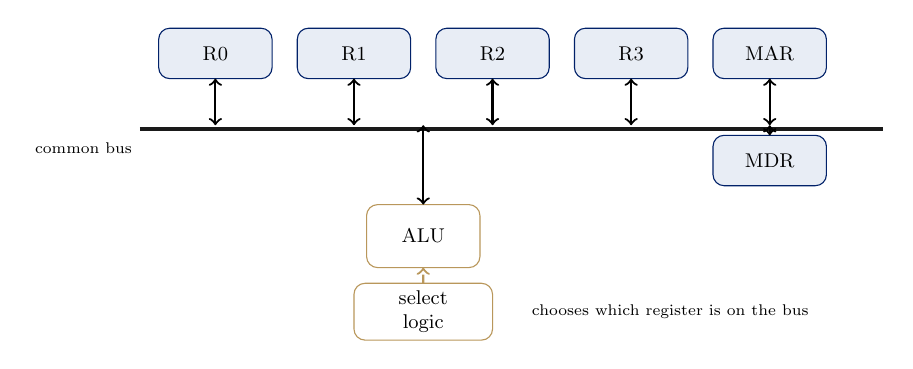
\begin{tikzpicture}[scale=0.80, transform shape,
        every node/.style={font=\small}]
      \draw[very thick, jet] (-1.2,0) -- (10.6,0);
      \node[font=\scriptsize, below left] at (-1.2,-0.1) {common bus};
      \node[draw=primary-blue, fill=light-bg, rounded corners,
            minimum width=1.8cm, minimum height=0.8cm, align=center] (R0) at (0,1.2) {R0};
      \node[draw=primary-blue, fill=light-bg, rounded corners,
            minimum width=1.8cm, minimum height=0.8cm, align=center] (R1) at (2.2,1.2) {R1};
      \node[draw=primary-blue, fill=light-bg, rounded corners,
            minimum width=1.8cm, minimum height=0.8cm, align=center] (R2) at (4.4,1.2) {R2};
      \node[draw=primary-blue, fill=light-bg, rounded corners,
            minimum width=1.8cm, minimum height=0.8cm, align=center] (R3) at (6.6,1.2) {R3};
      \foreach \x in {0, 2.2, 4.4, 6.6} { \draw[<->, thick] (\x,0.8) -- (\x,0.06); }
      \node[draw=primary-gold, fill=white, rounded corners,
            minimum width=1.8cm, minimum height=1.0cm, align=center] (ALU) at (3.3,-1.7) {ALU};
      \draw[<->, thick] (3.3,0.06) -- (3.3,-1.2);
      \node[draw=primary-blue, fill=light-bg, rounded corners,
            minimum width=1.8cm, minimum height=0.8cm, align=center] (MAR) at (8.8,1.2) {MAR};
      \node[draw=primary-blue, fill=light-bg, rounded corners,
            minimum width=1.8cm, minimum height=0.8cm, align=center] (MDR) at (8.8,-0.5) {MDR};
      \draw[<->, thick] (8.8,0.8) -- (8.8,0.06);
      \draw[<->, thick] (8.8,-0.1) -- (8.8,0.06);
      \node[draw=primary-gold, fill=white, rounded corners,
            minimum width=2.2cm, minimum height=0.8cm, align=center] (DEC) at (3.3,-2.9) {select\\logic};
      \draw[->, thick, primary-gold, dashed] (DEC.north) -- (3.3,-2.2);
      \node[font=\scriptsize, anchor=west] at (4.9,-2.9) {chooses which register is on the bus};
    \end{tikzpicture}
  \end{center}
  One shared path carries values among registers, ALU, and memory --- cf.~Mano,
  Fig.~5-4, p.129 (registers and memory on the common bus system)
  \cite{Mano1993_computer_system_architecture}. A \key{select} unit (decoder)
  chooses, each cycle, \emph{which} register drives the bus.
\end{frame}

\begin{frame}{Register-Selection Signals: SELA / SELB / SELD}
  \begin{block}{How a transfer picks its source and destination (Mano, Table 8-1, p.243)}
    \begin{itemize}
      \item \texttt{SELA} --- which register's contents go to the ALU's
        \emph{first} input.
      \item \texttt{SELB} --- which register's contents go to the ALU's
        \emph{second} input.
      \item \texttt{SELD} --- \emph{which} register is loaded with the result.
    \end{itemize}
  \end{block}
  \begin{exampleblock}{The idea}
    Register selection is just \emph{encoded} in a few select bits and decoded
    into one-hot ``drive bus'' / ``load now'' signals. That is the whole trick
    behind moving values between registers without hard-wiring every pair.
  \end{exampleblock}
\end{frame}

\begin{frame}{Worked Example: \texttt{R1} $\gets$ \texttt{[R2]} over the Bus}
  \begin{block}{Transfer request}
    Copy the \emph{contents} of \texttt{R2} into \texttt{R1} (notation: the
    contents of a register X are written $[X]$).
  \end{block}
  \begin{enumerate}
    \item \texttt{SELA} encodes ``\texttt{R2}'' --- R2's output enable goes high.
    \item \texttt{R2}'s contents are driven onto the common bus.
    \item \texttt{SELD} encodes ``\texttt{R1}'' --- R1's load-enable goes high.
    \item On the clock edge, \texttt{R1} captures whatever the bus holds:
      $R1 \gets [R2]$.
  \end{enumerate}
  \vspace{0.2cm}
  \muted{No direct R2$\to$R1 wire exists --- every transfer uses the bus plus two
  select signals. Same mechanism drives every register move and ALU operand.}
\end{frame}

\begin{frame}{Socratic Check: Why Not Put \emph{Everything} in Registers?}
  \begin{alertblock}{Question}
    If registers are the fastest storage, why does a program put \texttt{X},
    \texttt{A}, \texttt{B}, \texttt{C}, \texttt{D} in memory instead of keeping
    everything in \texttt{R0..Rn-1}?
  \end{alertblock}
  \begin{itemize}
    \item \bad{Registers are scarce}: a few dozen at most --- the program cannot
      keep megabytes of data there.
    \item \bad{Cost}: each register costs silicon area and consumes power; large
      register files are expensive.
    \item \good{Registers are a \emph{scratchpad} for what is \emph{being}
      worked on}: values rest in memory (big, cheap, persistent) and are loaded
      into registers only while the ALU touches them.
  \end{itemize}
\end{frame}

% =============================================================================
% ACT 2 --- STACK ORGANIZATION
% =============================================================================
\section{Stack Organization}

\transitionslide{Registers are the fast scratchpad. A stack is a different way to organize operands.}

\begin{frame}{Motivation: How Do You Evaluate a Postfix Expression?}
  \begin{block}{Socratic question}
    Humans write \texttt{A + B}; machines with one ALU must feed it two operands.
    How would a calculator evaluate \texttt{A B +} if it could only look at the
    \emph{top} item of a scratch list --- no registers, no random access?
  \end{block}
  \begin{itemize}
    \item The rule: read a value, \key{push} it; read an operator, \key{pop}
      the last two values, compute, \key{push} the result.
    \item The \emph{last} value pushed is the \emph{first} one taken back out ---
      \key{last-in, first-out} (LIFO). That is a \key{stack}.
    \item Many machines (HP calculators, the JVM) use exactly this model.
  \end{itemize}
\end{frame}

\begin{frame}{Definition: Stack, SP, PUSH/POP}
  \begin{block}{Stack}
    A \textbf{stack} is an ordered storage structure where all insertions and
    deletions happen at \emph{one end}, the \textbf{top}, addressed by a
    dedicated register \texttt{SP} (the \key{stack pointer}). Behavior is
    LIFO (Mano, Sec.~8-3, p.247) \cite{Mano1993_computer_system_architecture}.
  \end{block}
  \begin{itemize}
    \item \key{PUSH}: $SP \gets [SP] - 1$, then $M[SP] \gets$ operand --- store
      at the new top. (Stack grows \emph{downward} toward lower addresses.)
    \item \key{POP}: operand $\gets M[SP]$, then $SP \gets [SP] + 1$ --- remove
      the current top.
  \end{itemize}
  \begin{exampleblock}{Worked micro-transfer}
    Stack contains \texttt{[? , 5 , 7]}, top at 7. \texttt{PUSH 9}
    $\Rightarrow$ stack \texttt{[? , 5 , 7 , 9]}; \texttt{POP} $\Rightarrow$
    returns 9, stack back to \texttt{[? , 5 , 7]}.
  \end{exampleblock}
\end{frame}

\begin{frame}{Worked Example: \texttt{A + B} on a Stack Machine}
  \footnotesize
  \begin{tabular}{@{}clp{4.2cm}p{4.2cm}@{}}
    \toprule
    \textbf{Step} & \textbf{Operation} & \textbf{Stack after (top right)} & \textbf{Effect} \\
    \midrule
    1 & \texttt{PUSH A} & \texttt{A} & value A stored at top \\
    2 & \texttt{PUSH B} & \texttt{B A} & value B stored above A \\
    3 & \texttt{ADD}    & \texttt{A+B} & pop B, pop A, push result \\
    4 & \texttt{POP X}  & \emph{empty} & store top into \texttt{X} \\
    \bottomrule
  \end{tabular}
  \vspace{0.3cm}
  \begin{alertblock}{Notice}
    The \texttt{ADD} instruction names \emph{no operands at all} --- both come
    implicitly from the top of the stack. This is the \key{zero-address}
    instruction format we meet in Act~3.
  \end{alertblock}
\end{frame}

\begin{frame}{Register Stack vs.\ Memory Stack}
  \begin{block}{Two hardware homes for a stack (Mano, Sec.~8-3, p.248)}
    \begin{itemize}
      \item \key{Register stack}: the stack lives inside the CPU in a set of
        registers --- very fast, but only a handful of words (e.g.~64 words).
      \item \key{Memory stack}: the stack is a region of main memory, with
        \texttt{SP} holding the address of the current top --- as large as
        memory, but every PUSH/POP is a memory access.
    \end{itemize}
  \end{block}
  \begin{exampleblock}{Why real machines choose memory stacks}
    Function calls nest deeply (recursion); a few registers cannot hold the
    frames. Real ISAs keep \texttt{SP} in a register and store stack frames in
    memory --- registers are the pointer, memory is the stack.
  \end{exampleblock}
\end{frame}

\begin{frame}{Socratic Check: Registers vs.\ Stack as the Operand Home}
  \begin{alertblock}{Question}
    Both a register file and a stack can supply the ALU's operands. What does a
    stack force you to do that registers do not?
  \end{alertblock}
  \begin{itemize}
    \item \bad{Access is restricted}: you can only reach the \emph{top} --- no
      random access to \texttt{R0..Rn-1}-style slots mid-computation.
    \item \bad{Reordering costs}: to use a value that is buried, you must pop
      everything above it first (or shuffle).
    \item \good{But instructions shrink}: operands are implicit --- hence the
      compact \key{zero-address} format. Compilers love the compactness; hardware
      pays with restricted access.
  \end{itemize}
\end{frame}

% =============================================================================
% ACT 3 --- INSTRUCTION FORMATS
% =============================================================================
\section{Instruction Formats}

\transitionslide{The operand's home (registers, memory, stack) shapes what an instruction must say.}

\begin{frame}{Motivation: What Must an Instruction Say?}
  \begin{block}{Socratic question}
    The CPU must be told \emph{what} to do and \emph{where} the operands are.
    How much ``where'' information must a machine instruction physically carry?
  \end{block}
  \begin{itemize}
    \item Minimum: an \key{opcode} --- which operation (\texttt{ADD},
      \texttt{LOAD}, \dots).
    \item Beyond that: \emph{addresses} of operands and results --- and each
      address costs bits in the instruction word.
    \item The trade-off is fundamental: \key{more addresses per instruction}
      $\Rightarrow$ more work done per instruction but \key{longer instructions};
      fewer addresses $\Rightarrow$ compact but \key{more instructions} (and the
      hardware must know where the operands are implicitly).
  \end{itemize}
\end{frame}

\begin{frame}{Definition: Instruction Format}
  \begin{block}{Instruction format}
    An \textbf{instruction format} is the layout of an instruction word: an
    \textbf{opcode} field naming the operation, followed by zero or more
    \textbf{address/operand} fields naming where operands and results live
    (Mano, Sec.~8-4, p.255) \cite{Mano1993_computer_system_architecture}.
  \end{block}
  \begin{itemize}
    \item Fields are fixed-width bits; the opcode width sets an upper bound on
      how many distinct instructions the ISA can name.
    \item Address fields can name registers (short, cheap) or memory locations
      (long, flexible) --- Week 5 turns those fields into real addresses via
      \key{addressing modes}.
  \end{itemize}
\end{frame}

\begin{frame}{The Four Format Families}
  \begin{center}
    % Diagram: the four instruction-format families as horizontal word layouts.
    % Coordinates: (x, y) with scale 0.6
    %   Row 0 (3-address): rect x 0..10.4 at y 0.0, sep at 2.6/5.2/7.8
    %   Row 1 (2-address): rect x 0..7.8  at y -1.4, sep at 2.6/5.2
    %   Row 2 (1-address): rect x 0..5.2  at y -2.8, sep at 2.6
    %   Row 3 (0-address): rect x 0..2.6  at y -4.2, no sep
    %   Labels OP / R1..R3 centered in each field; names left of each row.
    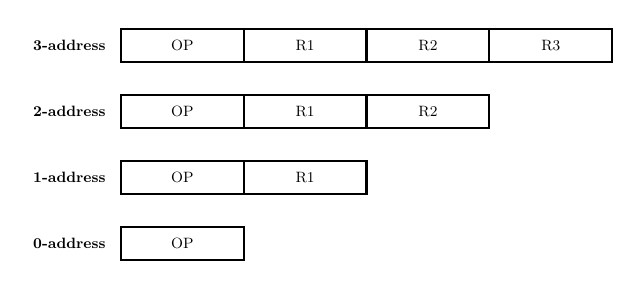
\begin{tikzpicture}[scale=0.6, transform shape,
        every node/.style={font=\small}]
      \draw[thick] (0,0) rectangle (10.4,-0.7);
      \draw[thick] (2.6,0) -- (2.6,-0.7);  \draw[thick] (5.2,0) -- (5.2,-0.7);
      \draw[thick] (7.8,0) -- (7.8,-0.7);
      \node at (1.3,-0.35) {OP}; \node at (3.9,-0.35) {R1};
      \node at (6.5,-0.35) {R2}; \node at (9.1,-0.35) {R3};
      \node[left] at (-0.2,-0.35) {\textbf{3-address}};
      \draw[thick] (0,-1.4) rectangle (7.8,-2.1);
      \draw[thick] (2.6,-1.4) -- (2.6,-2.1);  \draw[thick] (5.2,-1.4) -- (5.2,-2.1);
      \node at (1.3,-1.75) {OP}; \node at (3.9,-1.75) {R1}; \node at (6.5,-1.75) {R2};
      \node[left] at (-0.2,-1.75) {\textbf{2-address}};
      \draw[thick] (0,-2.8) rectangle (5.2,-3.5);
      \draw[thick] (2.6,-2.8) -- (2.6,-3.5);
      \node at (1.3,-3.15) {OP}; \node at (3.9,-3.15) {R1};
      \node[left] at (-0.2,-3.15) {\textbf{1-address}};
      \draw[thick] (0,-4.2) rectangle (2.6,-4.9);
      \node at (1.3,-4.55) {OP};
      \node[left] at (-0.2,-4.55) {\textbf{0-address}};
    \end{tikzpicture}
  \end{center}
  As the operand count falls, instructions get shorter but the machine must
  find operands \emph{implicitly} (accumulator or stack top).
\end{frame}

\begin{frame}{Three- and Two-Address Forms}
  \begin{block}{3-address: \texttt{ADD R1, R2, R3} $\Rightarrow$ $R1 \gets [R2]+[R3]$}
    Operands and destination are all explicit --- the most flexible, longest form.
  \end{block}
  \begin{block}{2-address: \texttt{ADD R1, R2} $\Rightarrow$ $R1 \gets [R1]+[R2]$}
    The first field doubles as one operand \emph{and} the result destination
    (\key{destructive} --- the old value of \texttt{R1} is lost).
  \end{block}
  \vspace{0.2cm}
  \muted{Fewer fields $\Rightarrow$ shorter instructions and smaller programs, at
  the cost of destroying one operand and needing explicit copy instructions.}
\end{frame}

\begin{frame}{One- and Zero-Address Forms}
  \begin{block}{1-address (accumulator): \texttt{ADD A} $\Rightarrow$ $AC \gets [AC]+[A]$}
    One operand is always the \key{accumulator} \texttt{AC}, named by no field;
    the single field names the other operand (usually memory).
  \end{block}
  \begin{block}{0-address (stack): \texttt{ADD} $\Rightarrow$ pop two, push sum}
    Both operands come from the stack top --- the format carries \emph{only} the
    opcode; every operand is implicit.
  \end{block}
  \vspace{0.2cm}
  \muted{Extreme compactness, but every non-stack access needs explicit
  \texttt{PUSH}/\texttt{POP} instructions.}
\end{frame}

\begin{frame}{Worked Example: \texttt{X = (A+B)$\times$(C+D)} --- 3-Address}
  \begin{block}{Three-address: 3 instructions, operands all named}
    \begin{itemize}
      \item \texttt{ADD R1, A, B} \quad $\Rightarrow$ $R1 \gets A + B$
      \item \texttt{ADD R2, C, D} \quad $\Rightarrow$ $R2 \gets C + D$
      \item \texttt{MUL X, R1, R2} \quad $\Rightarrow$ $X \gets R1 \times R2$
    \end{itemize}
  \end{block}
  \begin{exampleblock}{Tally}
    3 instructions; each carries three addresses --- wide words, but the program
    is short and needs no extra data movement.
  \end{exampleblock}
\end{frame}

\begin{frame}{Worked Example: Same Expression, 2-Address}
  \footnotesize
  \begin{block}{Two-address: 5 instructions --- destructive form needs copies}
    \begin{itemize}
      \item \texttt{MOV R1, A} \quad $R1 \gets A$ \hspace{0.5cm}(explicit copy, since \texttt{ADD} overwrites)
      \item \texttt{ADD R1, B} \quad $R1 \gets R1 + B$
      \item \texttt{MOV R2, C} \quad $R2 \gets C$
      \item \texttt{ADD R2, D} \quad $R2 \gets R2 + D$
      \item \texttt{MUL X, R1} \quad $X \gets R1 \times R2$ \hspace{0.3cm}(R2 is the implicit second operand)
    \end{itemize}
  \end{block}
  \begin{exampleblock}{Tally}
    5 instructions vs.\ 3 --- the 2-address format is cheaper per instruction
    but needs \key{extra copy instructions} because \texttt{ADD} is destructive.
  \end{exampleblock}
\end{frame}

\begin{frame}{Worked Example: Same Expression, 1- and 0-Address}
  \footnotesize
  \begin{block}{One-address (accumulator): 7 instructions, operands via \texttt{AC} + memory}
    \texttt{LOAD A; ADD B; STORE T; LOAD C; ADD D; MUL T; STORE X} --- with a
    temporary \texttt{T} in memory because the accumulator cannot hold two
    partial results at once.
  \end{block}
  \begin{block}{Zero-address (stack): 8 instructions, operands implicit}
    \texttt{PUSH A; PUSH B; ADD; PUSH C; PUSH D; ADD; MUL; POP X} --- shortest
    instructions, but the most of them.
  \end{block}
  \vspace{0.2cm}
  \muted{Same expression, four formats: 3, 5, 7, and 8 instructions. The format
  choice is a real, countable trade-off.}
\end{frame}

\begin{frame}{Instruction Formats: Side by Side}
  \footnotesize
  \setlength{\tabcolsep}{4pt}
  \begin{tabular}{@{}p{1.8cm}p{2.4cm}p{3.4cm}p{2.2cm}p{2.4cm}@{}}
    \toprule
    \textbf{Format} & \textbf{Example} & \textbf{Program size for} \\[-1pt]
    $X=(A{+}B)\times(C{+}D)$ & \textbf{Operand access} & \textbf{Typical use} \\
    \midrule
    3-address & \texttt{ADD R1,R2,R3} & 3 instr., wide words & all explicit & register ISAs (RISC) \\
    2-address & \texttt{ADD R1,R2}    & 5 instr. + copies     & one destroyed      & older CISC \\
    1-address & \texttt{ADD A}        & 7 instr., needs temps & accumulator        & simple CPUs \\
    0-address & \texttt{ADD}          & 8 instr., compact    & stack top          & stack machines, JVM \\
    \bottomrule
  \end{tabular}
  \vspace{0.3cm}
  \begin{center}
    \muted{More addresses per instruction $\Rightarrow$ fewer instructions but
    wider words; fewer addresses $\Rightarrow$ more instructions but compact.}
  \end{center}
\end{frame}

% =============================================================================
% ACT 4 --- INSTRUCTION CYCLE + TYPES OF OPERANDS
% =============================================================================
\section{Instruction Cycle}

\transitionslide{We have the storage spaces and the formats. Now: how does the CPU step one instruction?}

\begin{frame}{Motivation: Who Runs the Show, Step by Step?}
  \begin{block}{Socratic question}
    \texttt{ADD R1, A} sits in memory. For it to take effect, the CPU must bring
    the instruction in, understand it, collect \texttt{[R1]} and \texttt{[A]},
    add, and store back. What \emph{sequence of basic steps} does the machine
    repeat for \emph{every} instruction?
  \end{block}
  \begin{itemize}
    \item The answer is a fixed skeleton --- the \key{instruction cycle} --- that
      the control unit runs over and over, once per instruction.
    \item The skeleton is the \emph{same} for every instruction; only the
      \key{execute} phase differs by opcode.
  \end{itemize}
\end{frame}

\begin{frame}{The Instruction Cycle}
  \begin{center}
    % Diagram: the instruction cycle -- fetch, decode, execute -- as a loop.
    % Coordinates: (x, y), scale 0.85
    %   FETCH at (0,0)   DECODE at (4.6,0)  EXECUTE at (9.2,0)  (2.2w x 1.0h)
    %   boxes span y -0.5..0.5; sub-captions sit BELOW boxes at y=-0.85
    %   arrows: FETCH -> DECODE -> EXECUTE -> back to FETCH (top edge, y=1.3)
    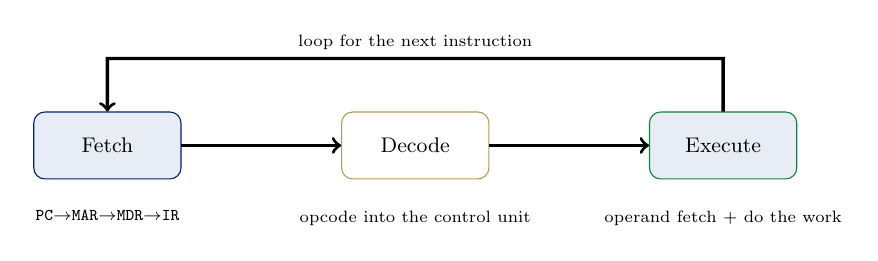
\begin{tikzpicture}[scale=0.85, transform shape,
        every node/.style={font=\small}]
      \node[draw=primary-blue, fill=light-bg, rounded corners,
            minimum width=2.2cm, minimum height=1.0cm, align=center] (F) at (0,0) {Fetch};
      \node[draw=primary-gold, fill=white, rounded corners,
            minimum width=2.2cm, minimum height=1.0cm, align=center] (D) at (4.6,0) {Decode};
      \node[draw=positive, fill=light-bg, rounded corners,
            minimum width=2.2cm, minimum height=1.0cm, align=center] (E) at (9.2,0) {Execute};
      \draw[->, very thick] (F.east) -- (D.west);
      \draw[->, very thick] (D.east) -- (E.west);
      \draw[->, very thick] (E.north) -- (9.2,1.3) -- (0,1.3) -- (F.north);
      \node[font=\scriptsize, above] at (4.6,1.3) {loop for the next instruction};
      \node[font=\scriptsize, below] at (0,-0.85) {\texttt{PC}$\to$\texttt{MAR}$\to$\texttt{MDR}$\to$\texttt{IR}};
      \node[font=\scriptsize, below] at (4.6,-0.85) {opcode into the control unit};
      \node[font=\scriptsize, below] at (9.2,-0.85) {operand fetch + do the work};
    \end{tikzpicture}
  \end{center}
  \vspace{0.2cm}
  Fetch $\to$ decode $\to$ execute is the standard instruction-cycle skeleton
  (Hamacher, \textit{Computer Organization}, Ch.~7; standard treatment)
  \cite{Hamacher2002_computer_organization}.
\end{frame}

\begin{frame}{The Fetch Phase, Step by Step}
  \footnotesize
  \begin{block}{Fetch transfers (\texttt{PC} knows where the next instruction lives)}
    \begin{itemize}
      \item \texttt{MAR} $\gets$ \texttt{[PC]} \quad --- remember the address.
      \item Initiate a memory \emph{read} at \texttt{MAR}.
      \item \texttt{MDR} $\gets$ \emph{memory data} \quad --- the instruction
        word comes back into the CPU.
      \item \texttt{IR} $\gets$ \texttt{[MDR]} \quad --- the instruction now
        sits in the instruction register.
      \item \texttt{PC} $\gets$ \texttt{[PC]} $+ 1$ \quad --- prepare the
        \emph{next} fetch.
    \end{itemize}
  \end{block}
  \begin{exampleblock}{Why these registers?}
    \texttt{PC} holds the next address, \texttt{MAR} pins it during the access,
    \texttt{MDR} buffers the incoming word, \texttt{IR} holds the current
    instruction while it is decoded. Each register exists for \emph{one} reason
    in the cycle.
  \end{exampleblock}
\end{frame}

\begin{frame}{The Decode and Execute Phases}
  \begin{block}{Decode}
    The opcode bits of \texttt{IR} tell the control unit \emph{which} operation
    this is --- the unit then selects the right sequence of control signals
    (exactly what we build in Weeks 6--7).
  \end{block}
  \begin{exampleblock}{Execute --- the operand-dependent part}
    \begin{itemize}
      \item If a memory operand is needed, its address is resolved (addressing
        modes, Week 5) and the operand fetched into a register.
      \item The ALU performs the operation; the result is written to the
        destination named in the instruction.
      \item The \emph{number} of execute steps varies by instruction --- fetch
        is fixed, execute is not.
    \end{itemize}
  \end{exampleblock}
\end{frame}

\begin{frame}{Worked Example: One Full Cycle for \texttt{ADD R1, A}}
  \footnotesize
  \begin{tabular}{@{}cp{3.4cm}p{3.6cm}p{3.4cm}@{}}
    \toprule
    \textbf{Phase} & \textbf{Register activity} & \textbf{Memory / ALU} & \textbf{State} \\
    \midrule
    Fetch &
      \texttt{MAR}$\gets$\texttt{[PC]}; \texttt{MDR}$\gets$instr.; \\
      \texttt{IR}$\gets$\texttt{[MDR]}; \texttt{PC}$\gets$\texttt{[PC]}$+1$ &
      read instruction word &
      instruction in \texttt{IR} \\
    Decode &
      \texttt{IR} opcode $\to$ control unit &
      --- &
      operation identified \\
    Execute &
      operand \texttt{[A]} fetched; \texttt{AC}$\gets$\texttt{[AC]}+\texttt{[A]} &
      read operand; ALU adds &
      result in \texttt{AC} \\
    \bottomrule
  \end{tabular}
  \vspace{0.3cm}
  \begin{alertblock}{Takeaway}
    The same three phases run for every instruction --- only the execute row
    changes. This is the loop the CPU is always inside.
  \end{alertblock}
\end{frame}

\begin{frame}{Types of Operands}
  \begin{block}{Fields an instruction can name (Hamacher, Ch.~7) \cite{Hamacher2002_computer_organization}}
    \begin{itemize}
      \item \key{Addresses}: a location in memory (used by \texttt{LOAD},
        \texttt{STORE}, \texttt{BRANCH}).
      \item \key{Numbers}: integer or floating-point values the ALU computes on.
      \item \key{Characters}: text --- usually ASCII/Unicode codes stored in a
        byte or halfword.
      \item \key{Logical data}: bit patterns --- each bit is its own value;
        operations like \texttt{AND}, \texttt{OR}, \texttt{XOR}, \texttt{shift}
        work bitwise.
    \end{itemize}
  \end{block}
  \begin{exampleblock}{Why this matters}
    The \emph{type} determines how the ALU wires the bits: a branch needs the
    address, an integer add needs the value, a shift needs the bit mask. The
    opcode says which interpretation applies.
  \end{exampleblock}
\end{frame}

\begin{frame}{Socratic Check: Tying the Week Together}
  \begin{alertblock}{Question}
    For \texttt{ADD R1, A} on an accumulator machine: which register holds the
    next instruction's address, which holds the current instruction, and where
    do the two operands of the ADD come from?
  \end{alertblock}
  \begin{itemize}
    \item \texttt{PC} points at the next instruction; \texttt{IR} holds the
      current one after fetch.
    \item First operand: \texttt{AC} (accumulator --- the implicit operand of
      the 1-address format).
    \item Second operand: memory location \texttt{A}, fetched during execute.
    \item Every piece of this answer came from Acts 1--4 --- the registers, the
      formats, and the cycle are one connected machine.
  \end{itemize}
\end{frame}

% =============================================================================
% ACT 5 --- SYNTHESIS
% =============================================================================
\section{Synthesis}

\transitionslide{One instruction, one cycle: registers hold, formats name, the cycle runs.}

\begin{frame}{The Three Threads Meet}
  \begin{block}{Storage spaces and formats are two sides of one choice}
    \begin{itemize}
      \item \key{Registers}: fast, explicit, random access --- buys the wide
        3-address format.
      \item \key{Stack}: compact, restricted, implicit --- buys the 0-address
        format.
      \item The instruction cycle is the \emph{glue}: it steps whichever format
        the ISA chose, through the same fetch/decode/execute skeleton.
    \end{itemize}
  \end{block}
  \begin{exampleblock}{The running thread, closed}
    $X = (A+B)\times(C+D)$ ran in 3, 5, 7, or 8 instructions depending on the
    format --- and each of those instructions then lives through one full
    fetch--decode--execute cycle.
  \end{exampleblock}
\end{frame}

\begin{frame}{Bridge to Week 5}
  \begin{block}{What we built today}
    \begin{itemize}
      \item The CPU's storage: registers (fast scratchpad), stack (LIFO operand
        home), memory (big and slow).
      \item Four instruction formats, with a counted cost per format.
      \item The fetch--decode--execute cycle and the four types of operands.
    \end{itemize}
  \end{block}
  \begin{exampleblock}{What's still missing}
    We wrote ``\texttt{ADD R1, A}'' and said ``operand \texttt{[A]} is
    fetched'' --- but we never said \key{how} the field \texttt{A} turns into the
    actual location of the operand. That is \key{addressing modes}, next week ---
    together with the datapath (buses) that actually moves the values.
  \end{exampleblock}
\end{frame}

\begin{frame}{Summary}
  \begin{itemize}
    \item \key{Register organization}: registers are the one-cycle scratchpad;
      transfers happen over a common bus selected by \texttt{SELA}/\texttt{SELB}/\texttt{SELD}.
    \item \key{Stack organization}: \texttt{SP} addresses a LIFO top; PUSH/POP
      with $\pm 1$ on \texttt{SP}; register stacks are fast, memory stacks are
      large.
    \item \key{Instruction formats}: 3-, 2-, 1-, 0-address --- the address count
      trades instruction width against program size (3 vs.\ 5 vs.\ 7 vs.\ 8
      instructions for one expression).
    \item \key{Instruction cycle}: fetch (\texttt{PC}$\to$\texttt{MAR}$\to$\texttt{MDR}$\to$\texttt{IR},
      \texttt{PC}${+}1$), decode, execute.
    \item \key{Operand types}: addresses, numbers, characters, logical data ---
      the opcode picks the interpretation.
  \end{itemize}
\end{frame}

\begin{frame}{References}
  \footnotesize
  \bibliographystyle{plain}
  \bibliography{../../Bibliography_base}
\end{frame}

\end{document}


